% Options for packages loaded elsewhere
\PassOptionsToPackage{unicode}{hyperref}
\PassOptionsToPackage{hyphens}{url}
%
\documentclass[
]{article}
\usepackage{lmodern}
\usepackage{amssymb,amsmath}
\usepackage{ifxetex,ifluatex}
\ifnum 0\ifxetex 1\fi\ifluatex 1\fi=0 % if pdftex
  \usepackage[T1]{fontenc}
  \usepackage[utf8]{inputenc}
  \usepackage{textcomp} % provide euro and other symbols
\else % if luatex or xetex
  \usepackage{unicode-math}
  \defaultfontfeatures{Scale=MatchLowercase}
  \defaultfontfeatures[\rmfamily]{Ligatures=TeX,Scale=1}
\fi
% Use upquote if available, for straight quotes in verbatim environments
\IfFileExists{upquote.sty}{\usepackage{upquote}}{}
\IfFileExists{microtype.sty}{% use microtype if available
  \usepackage[]{microtype}
  \UseMicrotypeSet[protrusion]{basicmath} % disable protrusion for tt fonts
}{}
\makeatletter
\@ifundefined{KOMAClassName}{% if non-KOMA class
  \IfFileExists{parskip.sty}{%
    \usepackage{parskip}
  }{% else
    \setlength{\parindent}{0pt}
    \setlength{\parskip}{6pt plus 2pt minus 1pt}}
}{% if KOMA class
  \KOMAoptions{parskip=half}}
\makeatother
\usepackage{xcolor}
\IfFileExists{xurl.sty}{\usepackage{xurl}}{} % add URL line breaks if available
\IfFileExists{bookmark.sty}{\usepackage{bookmark}}{\usepackage{hyperref}}
\hypersetup{
  pdftitle={Environmental DNA Metabarcoding for Simultaneous Monitoring and Ecological Assessment of Many Harmful Algae},
  pdfauthor={Emily Jacobs-Palmer; Ramón Gallego; Kelly Cribari; Abigail Keller; Ryan P. Kelly},
  hidelinks,
  pdfcreator={LaTeX via pandoc}}
\urlstyle{same} % disable monospaced font for URLs
\usepackage[margin=1in]{geometry}
\usepackage{longtable,booktabs}
% Correct order of tables after \paragraph or \subparagraph
\usepackage{etoolbox}
\makeatletter
\patchcmd\longtable{\par}{\if@noskipsec\mbox{}\fi\par}{}{}
\makeatother
% Allow footnotes in longtable head/foot
\IfFileExists{footnotehyper.sty}{\usepackage{footnotehyper}}{\usepackage{footnote}}
\makesavenoteenv{longtable}
\usepackage{graphicx,grffile}
\makeatletter
\def\maxwidth{\ifdim\Gin@nat@width>\linewidth\linewidth\else\Gin@nat@width\fi}
\def\maxheight{\ifdim\Gin@nat@height>\textheight\textheight\else\Gin@nat@height\fi}
\makeatother
% Scale images if necessary, so that they will not overflow the page
% margins by default, and it is still possible to overwrite the defaults
% using explicit options in \includegraphics[width, height, ...]{}
\setkeys{Gin}{width=\maxwidth,height=\maxheight,keepaspectratio}
% Set default figure placement to htbp
\makeatletter
\def\fps@figure{htbp}
\makeatother
\setlength{\emergencystretch}{3em} % prevent overfull lines
\providecommand{\tightlist}{%
  \setlength{\itemsep}{0pt}\setlength{\parskip}{0pt}}
\setcounter{secnumdepth}{-\maxdimen} % remove section numbering
\usepackage{gensymb}
\usepackage{fontspec}
\setmainfont{Open Sans}

\title{Environmental DNA Metabarcoding for Simultaneous Monitoring and
Ecological Assessment of Many Harmful Algae}
\author{Emily Jacobs-Palmer \and Ramón Gallego \and Kelly Cribari \and Abigail Keller \and Ryan P. Kelly}
\date{}

\begin{document}
\maketitle

\hypertarget{abstract}{%
\section{Abstract}\label{abstract}}

Harmful algae can have profound economic, environmental, and social
consequences. As the timing, frequency, and severity of harmful algal
blooms (HABs) change alongside global climate, efficient tools to
monitor and understand the current ecological context of these taxa are
increasingly important. Here we employ environmental DNA metabarcoding
to identify patterns in a wide variety of harmful algae and associated
ecological communities in the Hood Canal of Puget Sound in Washington
State, USA. We track trends of presence and abundance in a series of
water samples across nearly two years. We find putative harmful algal
sequences in a majority of samples, suggesting that these groups are
routinely present in local waters. We report patterns in variants of the
economically important genus \emph{Pseudo-nitzschia} (family
Bacillariaceae), as well as multiple harmful algal taxa previously
unknown or poorly documented in the region, including a cold-water
variant from the saxitoxin-producing genus \emph{Alexandrium} (family
Gonyaulacaceae), two variants from the karlotoxin-producing genus
\emph{Karlodinium} (family Kareniaceae), and one variant from the
parasitic genus \emph{Hematodinium} (family Syndiniaceae). We then use
data on environmental variables and the biological community surrounding
each algal taxon to illustrate the ecological context in which these
species are commonly found. Environmental DNA metabarcoding thus
simultaneously (1) alerts us to potential new or cryptic occurrences of
harmful algae, (2) expands our knowledge of the co-occurring conditions
and species associated with the growth of these organisms in changing
marine environments, and (3) provides a tool for monitoring and
management moving forward.

\hypertarget{introduction}{%
\section{Introduction}\label{introduction}}

Harmful algae and associated blooms create environmental, health, and
economic challenges at a global scale, causing mass die-offs in
ecosystems from de-oxygenation (Gobler, 2020; Griffith \& Gobler, 2020),
multiple types of poisoning in humans (Trainer et al., 2013), and
significant losses of revenue for the aquaculture industry (Trainer \&
Yoshida, 2014; Dìaz et al., 2019). For these reasons, local, national,
and international governing bodies organize and fund monitoring programs
to track HABs and identify the conditions that lead to their occurrence
(Graneli \& Lipiatou, 2002; Trainer, 2002; Lopez et al., 2008;
Moestrup). In addition, changing marine environments appear to be
causing increases in the duration, frequency, and severity of HABs
globally in association with rising temperatures and declining pH
(Gattuso et al., 2015a; Gobler et al., 2017).

Hood Canal, a natural glacial fjord within the Puget Sound of
Washington, USA, is a useful natural system in which to study the
ecology of harmful algae and likely future changes to their patterns of
occurrence. Surface temperatures of the region have risen 1.0°C since
the 1950s, dissolved oxygen levels are below 5 mg/L in deeper sections
of the sound, and pH has dropped by 0.05 - 0.15 units since
pre-industrial era (\textasciitilde1750) (Feely et al., 2010; Busch,
Harvey \& McElhany, 2013; Mauger et al., 2015). Warmer temperatures and
longer durations of warm conditions will create larger windows of growth
for HABs moving forward (Moore, Mantua \& Salathe Jr, 2011; Mauger et
al., 2015), with ocean acidification exacerbating the impacts of these
blooms by further increasing the toxicity and growth of harmful algal
species (Fu, Tatters \& Hutchins, 2012; Field et al., 2014).

Harmful algae fall into four primary categories: diatoms,
dinoflagellates, haptophytes, and raphidophytes. Of particular concern
locally are diatoms from the genus \emph{Pseudo-nitzschia} and
dinoflagellates from the genera \emph{Alexandrium}, \emph{Gonyaulax},
and \emph{Protoceratium}, each of which produces toxins that can
accumulate in shellfish grazers (Shimizu et al., 1975; Satake, MacKenzie
\& Yasumoto, 1998; Cembella, Lewis \& Quilliam, 2000; Trainer et al.,
2009, 2016). When consumed by humans, the toxins then cause symptoms
ranging from amnesia to paralysis, and can be deadly (Ferrante et al.,
2013; Grattan, Holobaugh \& Morris Jr, 2016). Additional harmful alga of
concern are fish-killing species such as the diatom \emph{Chaetoceros
concavicornis} and the raphidophyte \emph{Heterosigma akashiwo} (Yang \&
Albright, 1994; Khan, Arakawa \& Onoue, 1997). There is no current
ensemble testing protocol for all of these local problematic algae, and
both human-mediated transport and warming-related range shifts are
likely to introduce additional taxa. For example, there is recent
evidence that the toxic dinoflagellate \emph{Karenia mikimotoi} (family
Kareniaceae; described from Japan and also occurring in the North
Atlantic) is now present along the west coast of North America,
specifically off of Alaska and California (National Centers for Coastal
Ocean Science, 2014).

Because the effects of harmful algae are wide-ranging and potentially
devastating (Lewitus et al., 2012; Moore et al., 2019), monitoring of
these organisms and the environmental conditions with which they are
associated has long been a public health priority in Puget Sound and in
many locations around the world. Efforts to track blooms of these algae
have historically relied on the work of skilled taxonomists using
microscopic visual analysis of cells to identify species (e.g.~Lapworth,
Hallegraeff \& Ajani, 2001; Yang et al., 2000). More recently, satellite
spectrographic data (Tomlinson et al., 2004; Ahn et al., 2006),
molecular assays for toxins (Pierce \& Kirkpatrick, 2001; Murray et al.,
2011), and flow cytometry coupled with machine learning (Campbell et
al., 2010) have been employed to detect and track harmful algae.

Adding to the list of technological advances for monitoring are two
types of genetic techniques that rely on environmental DNA (eDNA)
present in the water to classify and assess the abundance of harmful
algae: quantitative Polymerase Chain Reaction (qPCR) and DNA
metabarcoding (Al-Tebrineh et al., 2010; Erdner et al., 2010; Antonella
\& Luca, 2013; Grzebyk et al., 2017; Ruvindy et al., 2018). The former
method tracks known taxa individually and requires substantial sequence
data to design species-specific primers and/or probes; the latter method
involves PCR with less-specific primers to generate amplicons from a
broad swath of taxa at a common locus. This second method,
metabarcoding, allows detection and even quantification of many taxa
simultaneously.

Because the specific target organisms need not be chosen \emph{a
priori}, metabarcoding may uncover taxa unexpected in the study region,
and in addition, can reveal a cross-section of the biological community
surrounding any particular group of interest (Deiner et al., 2017;
Taberlet et al., 2018). Previous work has described the ecological
context of harmful algae and their blooms using environmental covariates
(e.g.~Wells et al., 2015; Banerji et al., 2019), as well as assessments
of bloom-associated taxa (typically other microorganisms or viruses)
(e.g.~Loureiro et al., 2011; Buskey, 2008), although the labor required
for traditional survey methodology has limited the breadth of contextual
taxa included in these studies.

Here, we couple environmental monitoring with eDNA metabarcoding to
track the presence of dozens of potential harmful algal taxa
simultaneously, including a number unexpected or understudied in the
region of interest. Because of their economic and public-health
importance, we focus on variants in the genera \emph{Alexandrium}
(dinoflagellate family Gonyaulacaceae), \emph{Hematodinium}
(dinoflagellate family Syndiniaceae), \emph{Karlodinium} (dinoflagellate
family Kareniaceae), and \emph{Pseudo-nitzschia} (diatom family
Bacillariaceae), and examine the distribution of these in time and space
across 19 months of sampling at ten locations in Hood Canal. We model
the associations of individual algal lineages with key environmental
variables, and subsequently improve the predictive value of these models
by including co-occurring (non-algal) taxa as possible indicator
species. With these analyses, we present useful information on the
distributions and ecological contexts of potentially harmful algae in
the Puget Sound region, and demonstrate how eDNA metabarcoding can
improve our understanding and management of harmful algae, both locally
and globally.

\hypertarget{materials-and-methods}{%
\section{Materials and Methods}\label{materials-and-methods}}

\hypertarget{environmental-dna-sampling-and-measuring-environmental-variables}{%
\subsection{Environmental DNA Sampling and Measuring Environmental
Variables}\label{environmental-dna-sampling-and-measuring-environmental-variables}}

To identify a broad range of potential harmful algal taxa and
simultaneously survey the surrounding biological community, we sampled
seawater for eDNA from ten sites within Hood Canal, a natural glacial
fjord in Puget Sound, Washington, USA. Five sampling sites were
intertidal, and five were nearby nearshore locations at the approximate
center of the fjord. For intertidal locations at Salisbury Point County
Park (SA), Triton Cove State Park (TR), Lilliwaup Tidelands State Park
(LL), Potlatch State Park (PO), and Twanoh State Park (TW) (see Figure 1
and Table S1 for location coordinates), we collected three 1 L samples
of water from immediately below the surface using a bleach-cleaned
plastic bottle held at the end of a 1.7 meter pole. We sampled
intertidal locations every 1-2 months for approximately 1.5 years
between March 2017 and July 2018 (see Table S1 for sampling dates). At
these same stations and simultaneous with eDNA sampling, we collected
one 120 ml water sample from each site and poisoned it with 0.1 ml of
saturated HgCl\({_2}\) for carbonate chemistry analysis including pH,
following {[}REFREF{]}. We also collected in situ measurements of
temperature and salinity using a handheld multiprobe (Hanna Instruments,
USA) and a portable refractometer. We characterized sample carbonate
chemistry by measuring Total Alkalinity (TA; open-cell automated
titration based on a Dosimat plus (Metrohm AG) as part of a custom
system assembled by Andrew Dickson (University of California San Diego)
and used in the laboratory of Alex Gagnon at the University of
Washington) and Dissolved Inorganic Carbon (DIC; Apollo Instruments,
USA; CO2 extraction system with 10\% (v/v) phosphoric acid). Both
measurements were calibrated and validated with certified reference
material from the Scripps Oceanographic Institute. Using DIC and TA, we
calculated pH and the remaining carbonate system parameters with the R
package `seacarb` (Gattuso et al., 2015b), removing a single sample from
the dataset used for environmental modeling (see below) due to an
unreasonably low pH value (\textless7.5).

For nearshore locations, we sampled a selection of stations (P8, P14,
P12, P11, P402) surveyed by the Washington Ocean Acidification Center
during triannual cruises (see Figure 1 and Table S1 for location
coordinates). The samples used here were collected in September 2017 (2
samples), April 2018 (3 samples), and September 2018 (3 samples); See
Table S1 for sampling dates), by deploying a CTD with twelve Niskin
bottles at each station, and collecting data on temperature, salinity,
and pH (Alin) in addition to water for eDNA from immediately below the
surface. We filtered 500 mL of each water sample for eDNA from both
intertidal and nearshore locations with a cellulose acetate filter (47
mm diameter, 0.45 \(\mu\)m pore size), and preserved this filter in
Longmire buffer until DNA extraction (Kelly, Gallego \& Jacobs-Palmer,
2018). Many unmeasured variables influence planktonic communities (e.g.,
nutrients, sunlight, and wave energy); nevertheless the minimal set of
parameters we analyzed here clearly distinguished communities and was
adequate for the purposes of assessing temporal and spatial trends. Our
purpose was to describe patterns of harmful algae over space and time,
along with the environmental and ecological contexts in which they
occurred, rather than to test any particular mechanism by which harmful
algal taxa might respond to different environmental parameters.

\begin{figure}
\centering
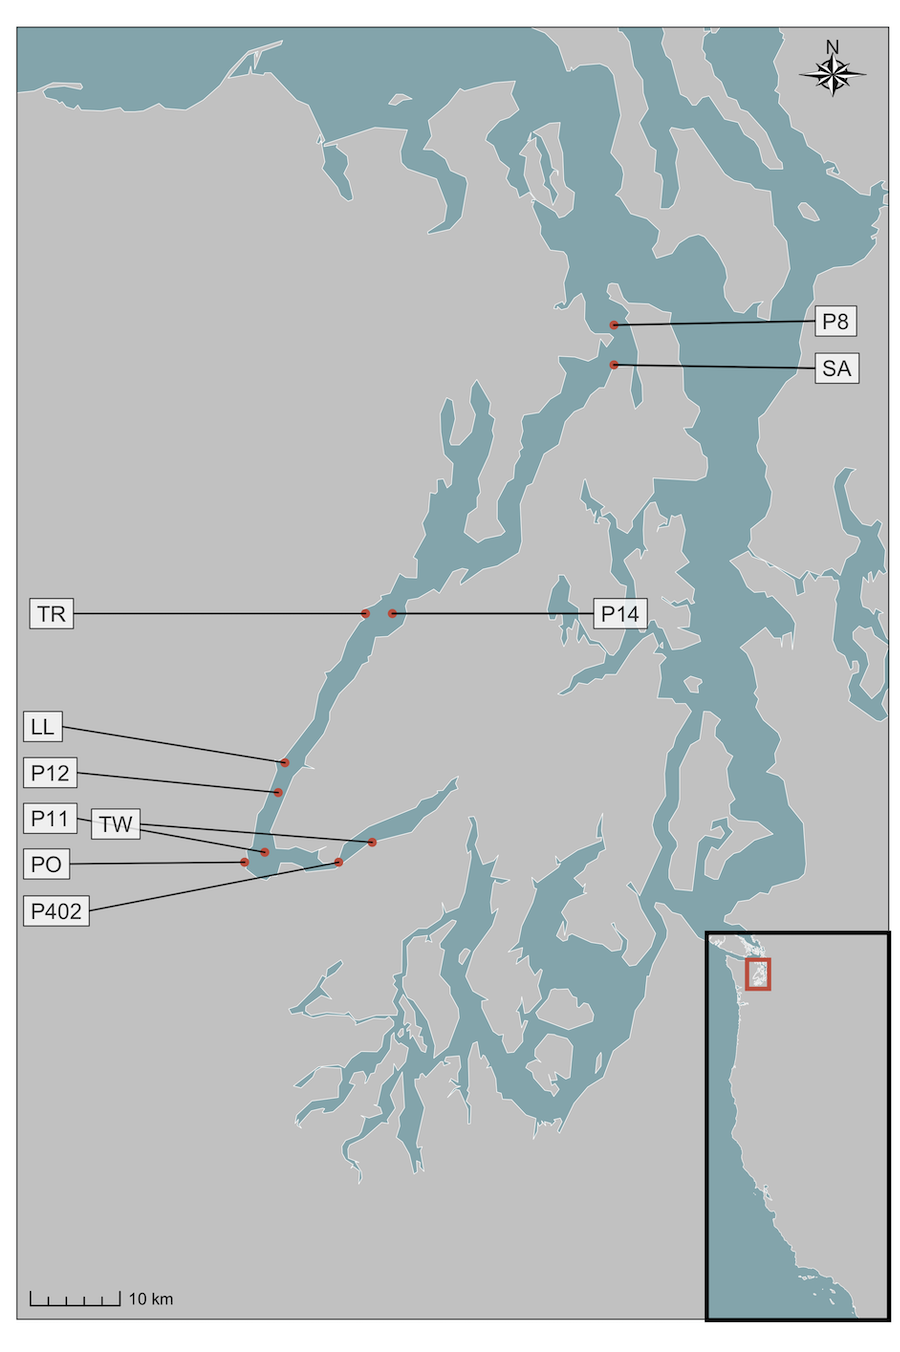
\includegraphics{../figures/SiteMap_small.png}
\caption{\label{fig:sitemap} Figure 1: Intertidal and nearshore sampling
locations in Hood Canal, Washington, USA. Site abbreviations are
described in the text, and coordinates are given in Table S1.}
\end{figure}

\hypertarget{extraction-amplification-and-sequencing}{%
\subsection{Extraction, Amplification, and
Sequencing}\label{extraction-amplification-and-sequencing}}

To extract DNA from sample filters, we used a phenol:chloroform:isoamyl
alcohol protocol (modified from Renshaw et al., 2015). To maximize
extraction efficiency and minimize co-extraction of inhibitors, we
incubated filter membranes at 65\(^\circ\)C for 30 min before adding 900
\(\mu\)L of phenol:chloroform:isoamyl alcohol and shaking vigorously for
60 s. We conducted two consecutive chloroform washes by centrifuging at
14,000 rpm for 5 min, transferring the aqueous layer to 700 \(\mu\)L
chloroform, and shaking vigorously for 60 s. After a third
centrifugation, we transferred 500 \(\mu\)L of the aqueous layer to
tubes containing 20 \(\mu\)L 5 molar NaCl and 500 \(\mu\)L 100\%
isopropanol, and froze these at −20\(^\circ\)C for approximately 15 h.
Finally, we centrifuged samples at 14,000 rpm for 10 min, poured off or
pipetted out any remaining liquid, and dried in a vacuum centrifuge at
45\(^\circ\)C for 15 min. We resuspended the eluate in 200 \(\mu\)L
water, and used 1 \(\mu\)L of diluted DNA extract (between 1:10 and
1:400) as template for PCR.

To identify a wide variety of metazoan taxa including putative harmful
algae and their surrounding biological communities from eDNA, we
amplified a \textasciitilde315 base pair segment of the Cytochrome
Oxidase I (COI) using universal primers described in Leray et al.
(2013). To distinguish technical from biological variance and to
quantify each, we ran and sequenced in triplicate PCR reactions from
each of the samples (i.e., individual bottles of water). For multiplex
sequencing on an Illumina MiSeq, we followed a two-step PCR protocol
(O'Donnell et al., 2016) with redundant 3' and 5' indexing. In the first
step, we used a PCR reaction containing 1X HotStar Buffer, 2.5 mM MgCl2,
0.5 mM dNTP, 0.3 \(\mu\)M of each primer, and 0.5 units of HotStar Taq
(Qiagen Corp., Valencia, CA, USA) per 20 \(\mu\)L reaction. The PCR
protocol for this step consisted of 40 cycles, including an annealing
touchdown from 62\(^\circ\)C to 46\(^\circ\)C (-1\(^\circ\)C per cycle),
followed by 25 cycles at 46\(^\circ\)C. In the second step, we added
identical 6 base-pair nucleotide tags to both ends of our amplicons,
with unique index sequences for each individual PCR reaction. We allowed
for no sequencing error in these tags; only sequences with identical
tags on both the forward and reverse read-directions survived quality
control. This gave us high confidence in assigning amplicons back to
individual field samples.

We generated amplicons with the same replication scheme for positive
control kangaroo (genus \emph{Macropus}) tissue, selected because this
genus is absent from the sampling sites and common molecular biology
reagents, but amplifies well with the universal primer set used in this
study. We could therefore use positive control samples to identify
possible cross-contamination: reads from other taxa that appear in these
samples allow us to estimate and account for the proportion of sequences
that are present in the incorrect PCR reaction (see Bioinformatics
below). We also amplified negative controls (molecular grade water) in
triplicate alongside environmental samples and positive controls, and
verified by gel electrophoresis that these PCR reactions contained no
appreciable amount of DNA (see Kelly, Gallego \& Jacobs-Palmer, 2018 for
a discussion of the merits of sequencing positive and not negative
controls).

To prepare libraries of replicated, indexed samples and positive
controls, we followed manufacturers' protocols (KAPA Biosystems,
Wilmington, MA, USA; NEXTflex DNA barcodes; BIOO Scientific, Austin, TX,
USA). We then performed sequencing on an Illumina MiSeq (250-300 bp,
paired-end) platform in seven different sets of samples: six for the
intertidal dataset and one for the nearshore dataset.

\hypertarget{bioinformatics}{%
\subsection{Bioinformatics}\label{bioinformatics}}

We followed updated versions of previously published procedures for
bioinformatics, quality control, and decontamination (Kelly, Gallego \&
Jacobs-Palmer, 2018). This protocol uses a custom Unix-based script
(Gallego) calling third-party programs to perform initial quality
control on sequence reads from all four runs combined, demultiplexing
sequences to their sample of origin and clustering unique variants into
amplicon sequence variants (ASVs) (Martin, 2011; Callahan et al., 2016).

Specifically, to address possible cross-sample contamination (see
Schnell, Bohmann \& Gilbert, 2015), we subtracted the maximum
proportional representation of each ASV across all positive control
samples (see Extraction, Amplification, and Sequencing above) from the
respective ASV in field samples. We estimated the probability of ASV
occurrence by performing occupancy modeling ({\textbf{???}}; Royle \&
Link, 2006). Following Lahoz-Monfort et al.~(2016) and using the full
Bayesian code for package rjags (Plummer et al., 2016) provided by those
authors, we modeled the probability of occupancy (i.e., true presence)
for each of the unique sequence variants in our dataset. We treated
replicate PCR reactions of each water bottle as independent trials,
estimating the true-positive rate of detection (\(P_{11}\)),
false-positive rate (\(P_{10}\)), and commonness (psi, \(\psi\)) in a
binomial model. We then used these parameters to estimate the overall
likelihood of occupancy (true presence) for each ASV; those with low
likelihoods (\textless80\%) were deemed unlikely to be truly present in
the dataset, and therefore culled. We removed samples whose PCR
replicates were highly dissimilar by calculating the Bray-Curtis
dissimilarity amongst PCR replicates from the same bottle of water and
discarding those with distance to the sample centroid outside a 95\%
confidence interval. The result was a dataset of \(3.98 * 10^{8}\) reads
from 5275 unique ASVs. Lastly, to collapse variants likely due to PCR
error, we converted ASVs to operational taxonomic units (OTUs) by
clustering with SWARM (Mahé et al., 2015). All bioinformatic and
analytical code is included in GitHub repositories {[}REFREF{]},
including the details of parameter settings in the bioinformatics
pipelines used. Sequence and annotation information are included as
well, and the former are deposited and publicly available in GenBank
(upon acceptance; accession numbers will be provided in the published
manuscript).

\hypertarget{taxonomy}{%
\subsection{Taxonomy}\label{taxonomy}}

We performed the taxonomic identification using a CRUX-generated
database for the Leray fragment of the COI gene (see Extraction,
Amplification, and Sequencing above), querying that database with a
Bowtie2 algorithm (as described in Curd et al., 2019). The algorithm
classifies the query sequence to the last common ancestor of ambiguously
classified sequences. Only matches with a bootstrap support greater than
90\% were kept. Here, we assigned taxonomy at the level of genus, rather
than species, for two main reasons. First, for some taxa, variation may
not be sufficient to distinguish species within a genus, and second,
representation of local species in the databases used may not be
complete, leading to the mis-assignment of sequences to their nearest
represented neighbor. We denoted different lineages within genera using
three-character abbreviation derived from the sequence variants
themselves. Full sequences for each variant are provided in Table S2. To
assess similarity of putative harmful algal lineages, we translated
nucleotide sequences with the ExPASy Bioinformatics Resource Portal
Translate tool using the mold, protozoan, and coelenterate
mitochondrial, mycoplasma/spiroplasma genetic code (Gasteiger et al.,
2003). We created both nucleotide and amino acid alignments with the
Clustal Omega Multiple Sequence Alignment tool (Sievers \& Higgins,
2014).

\hypertarget{species-distributions-in-space-and-time}{%
\subsection{Species Distributions in Space and
Time}\label{species-distributions-in-space-and-time}}

To examine the distribution of potential harmful algal taxa in time and
space, we calculated an index of relative eDNA abundance (hereafter eDNA
abundance index). To derive this index, we first normalized
taxon-specific ASV counts into proportions within a technical replicate,
and then transformed the proportion values such that the maximum across
all samples was scaled to 1 for each taxon (Kelly, Shelton \& Gallego,
2019). Such indexing allowed us to track trends in abundance of taxa in
time and space by correcting for both differences in read depth among
samples and differences in amplification efficiency among sequences
(mathematically, it is equivalent to the Wisconsin
double-standardization for community ecology as implemented in the vegan
package for R (Oksanen et al., 2013)). We plotted the eDNA abundance
index for each potential harmful algal taxon across all sampling events
from both intertidal and nearshore eDNA collections in our time series
between March 2017 and September 2018.

\hypertarget{environmental-and-biological-context}{%
\subsection{Environmental and Biological
Context}\label{environmental-and-biological-context}}

To explore the ways in which environmental variables were associated
with the presence or absence of our focal harmful algal taxa, we
compared logistic-regression models using taxon presence as outcome, and
combinations of three environmental variables (temperature, pH, and
salinity) as predictors. We also fit a variety of models in a Bayesian
hierarchical framework, where the slopes of predictors and intercepts
could vary by season (summer/winter), and included all models
(hierarchical and non-hierarchical) in our model comparison. Rather than
mechanically testing all possible combinations of models, we proposed
models that were reasonable given the observed patterns of occurrences;
in total, this resulted in between five and 17 models per taxon. For
purposes of the models, we designated April through September as being
``summer'', and other months ``winter''. Given many possible predictor
variables, developing a useful model without overfitting can be a
challenge. To combat this, we compared models using the widely
applicable information criterion (WAIC) (Watanabe, 2010), which makes no
assumptions about the shape of the posterior probability distribution
and -- like information criteria in general -- penalizes more complex
models. Moreover, WAIC quickly approximates the results of leave-one-out
cross-validation (McElreath, 2020) to estimate out-of-sample model
performance. Following model selection using WAIC, we reported the
in-sample model accuracy for reference.

To determine the species most closely associated with potential harmful
algal taxa, we performed canonical analysis of principal coordinates
(CAP) for each focal variant by implementing the capscale function in
vegan (Oksanen et al., 2013), which revealed the degree to which other
taxa in the surrounding biological communities could be associated with
presence (versus absence) of the potential harmful algal taxon. Using
this ordination technique avoids the problem of testing each
co-occurring taxon for significant associations with our focal putative
harmful algae, thereby removing the need to statistically correct for
multiple comparisons. We then used these putative indicator taxa as
predictors in a second round of logistic regressions, adding only the
single most-strongly associated taxon as a separate intercept term to
the best-fit environmental models for each of our focal lineages
(above). Such contextual ecological information is useful to the extent
that it helps to predict the occurrence of harmful algal lineages
without overfitting, which we evaluated as described above using WAIC.

\hypertarget{results}{%
\section{Results}\label{results}}

\hypertarget{taxonomy-1}{%
\subsection{Taxonomy}\label{taxonomy-1}}

Environmental DNA metabarcoding of 63 samples from five intertidal and
five nearshore locations in Hood Canal, Washington, United States
revealed a total of 605 unique amplicon sequence variants (ASVs) for
which we were able to assign taxonomy to 262 distinct genera. Of these,
exactly 100 ASVs were assigned to genera that are known to contain
harmful algae (Horner \& Postel, 1993; Horner, Garrison \& Plumley,
1997; Trainer et al., 2016; Moestrup). These potential harmful algal
taxa are members of four main taxonomic groups -- diatoms,
dinoflagellates, haptophytes, and raphidophytes -- and represent
seventeen genera (diatoms: \emph{Chaetoceros}, \emph{Nitzschia},
\emph{Pseudo-nitzschia}; dinoflagellates: \emph{Alexandrium},
\emph{Dinophysis}, \emph{Gonyaulax}, \emph{Gymnodinium (Akashiwo)},
\emph{Hematodinium}, \emph{Heterocapsa}, \emph{Karlodinium},
\emph{Prorocentrum}, \emph{Woloszynskia}; haptophytes:
\emph{Chrysocromulina}, \emph{Phaeocystis}; raphidophytes:
\emph{Chattonella}, \emph{Heterosigma}, \emph{Pseudochattonella}; See
Table S2 for a complete list of potential harmful algal taxonomic
assignments and COI sequences).

Taxa that occur rarely lack sufficient numbers of observations to allow
robust tests for association with environmental variables. Consequently,
we focus hereafter on the ASVs present in at least ten percent of
samples (minimum 7 occurrences out of 63 samples), an adequate sample
size to compare with environmental variables and biological context.
This subset of sequences included 191 total variants, 37 of which belong
to potentially harmful algal taxa (Table 1), and the rest to other
members of the biological community. These putative harmful algal
variants belong to 12 genera containing differing degrees of sequence
variation, with some such as \emph{Hematodinium} represented by a single
DNA and protein sequence, and others such as \emph{Nitzschia}
represented by a much larger number of DNA (10) and amino acid (5)
variants. Each of the potential harmful algal genera represented here
exhibit varying degrees and types of toxicity or harm, ranging from
physical irritation of fish gill tissue to production of toxins
dangerous to human health (Table 1; Trainer et al., 2016; Simonsen \&
Moestrup, 1997; Lindberg, Moestrup \& Daugbjerg, 2005; Stentiford \&
Shields, 2005; Kotaki et al., 2006; Peperzak \& Poelman, 2008; Skjelbred
et al., 2011; Place et al., 2012; Cho et al., 2017).

\smallsize

\begin{longtable}[]{@{}cccccc@{}}
\caption{Table 1: Potential harmful algal taxa identified by eDNA in at
least ten percent of samples from in Hood Canal, WA. Type of harmful
algae and genus are given, as well as the number of DNA and protein
variants, toxicity, and sampling location(s) for member(s) of that
genus. \normalsize }\tabularnewline
\toprule
\begin{minipage}[b]{0.11\columnwidth}\centering
Type\strut
\end{minipage} & \begin{minipage}[b]{0.13\columnwidth}\centering
Genus\strut
\end{minipage} & \begin{minipage}[b]{0.10\columnwidth}\centering
DNA variants\strut
\end{minipage} & \begin{minipage}[b]{0.13\columnwidth}\centering
Protein variants\strut
\end{minipage} & \begin{minipage}[b]{0.20\columnwidth}\centering
Toxicity (target)\strut
\end{minipage} & \begin{minipage}[b]{0.16\columnwidth}\centering
Sampling Location\strut
\end{minipage}\tabularnewline
\midrule
\endfirsthead
\toprule
\begin{minipage}[b]{0.11\columnwidth}\centering
Type\strut
\end{minipage} & \begin{minipage}[b]{0.13\columnwidth}\centering
Genus\strut
\end{minipage} & \begin{minipage}[b]{0.10\columnwidth}\centering
DNA variants\strut
\end{minipage} & \begin{minipage}[b]{0.13\columnwidth}\centering
Protein variants\strut
\end{minipage} & \begin{minipage}[b]{0.20\columnwidth}\centering
Toxicity (target)\strut
\end{minipage} & \begin{minipage}[b]{0.16\columnwidth}\centering
Sampling Location\strut
\end{minipage}\tabularnewline
\midrule
\endhead
\begin{minipage}[t]{0.11\columnwidth}\centering
Diatom\strut
\end{minipage} & \begin{minipage}[t]{0.13\columnwidth}\centering
Chaetoceros\strut
\end{minipage} & \begin{minipage}[t]{0.10\columnwidth}\centering
8\strut
\end{minipage} & \begin{minipage}[t]{0.13\columnwidth}\centering
5\strut
\end{minipage} & \begin{minipage}[t]{0.20\columnwidth}\centering
Gill irritation (finfish)\strut
\end{minipage} & \begin{minipage}[t]{0.16\columnwidth}\centering
Intertidal; Nearshore\strut
\end{minipage}\tabularnewline
\begin{minipage}[t]{0.11\columnwidth}\centering
Diatom\strut
\end{minipage} & \begin{minipage}[t]{0.13\columnwidth}\centering
Nitzschia\strut
\end{minipage} & \begin{minipage}[t]{0.10\columnwidth}\centering
10\strut
\end{minipage} & \begin{minipage}[t]{0.13\columnwidth}\centering
5\strut
\end{minipage} & \begin{minipage}[t]{0.20\columnwidth}\centering
Domoic acid and derivatives (human)\strut
\end{minipage} & \begin{minipage}[t]{0.16\columnwidth}\centering
Intertidal\strut
\end{minipage}\tabularnewline
\begin{minipage}[t]{0.11\columnwidth}\centering
Diatom\strut
\end{minipage} & \begin{minipage}[t]{0.13\columnwidth}\centering
Pseudo-nitzschia\strut
\end{minipage} & \begin{minipage}[t]{0.10\columnwidth}\centering
3\strut
\end{minipage} & \begin{minipage}[t]{0.13\columnwidth}\centering
2\strut
\end{minipage} & \begin{minipage}[t]{0.20\columnwidth}\centering
Domoic Acid (human)\strut
\end{minipage} & \begin{minipage}[t]{0.16\columnwidth}\centering
Intertidal; Nearshore\strut
\end{minipage}\tabularnewline
\begin{minipage}[t]{0.11\columnwidth}\centering
Dinoflagellate\strut
\end{minipage} & \begin{minipage}[t]{0.13\columnwidth}\centering
Alexandrium\strut
\end{minipage} & \begin{minipage}[t]{0.10\columnwidth}\centering
2\strut
\end{minipage} & \begin{minipage}[t]{0.13\columnwidth}\centering
2\strut
\end{minipage} & \begin{minipage}[t]{0.20\columnwidth}\centering
Saxitoxin (human)\strut
\end{minipage} & \begin{minipage}[t]{0.16\columnwidth}\centering
Intertidal; Nearshore\strut
\end{minipage}\tabularnewline
\begin{minipage}[t]{0.11\columnwidth}\centering
Dinoflagellate\strut
\end{minipage} & \begin{minipage}[t]{0.13\columnwidth}\centering
Hematodinium\strut
\end{minipage} & \begin{minipage}[t]{0.10\columnwidth}\centering
1\strut
\end{minipage} & \begin{minipage}[t]{0.13\columnwidth}\centering
1\strut
\end{minipage} & \begin{minipage}[t]{0.20\columnwidth}\centering
Parasitism (crab)\strut
\end{minipage} & \begin{minipage}[t]{0.16\columnwidth}\centering
Intertidal\strut
\end{minipage}\tabularnewline
\begin{minipage}[t]{0.11\columnwidth}\centering
Dinoflagellate\strut
\end{minipage} & \begin{minipage}[t]{0.13\columnwidth}\centering
Heterocapsa\strut
\end{minipage} & \begin{minipage}[t]{0.10\columnwidth}\centering
2\strut
\end{minipage} & \begin{minipage}[t]{0.13\columnwidth}\centering
2\strut
\end{minipage} & \begin{minipage}[t]{0.20\columnwidth}\centering
Haemolysis (shellfish)\strut
\end{minipage} & \begin{minipage}[t]{0.16\columnwidth}\centering
Intertidal; Nearshore\strut
\end{minipage}\tabularnewline
\begin{minipage}[t]{0.11\columnwidth}\centering
Dinoflagellate\strut
\end{minipage} & \begin{minipage}[t]{0.13\columnwidth}\centering
Karlodinium\strut
\end{minipage} & \begin{minipage}[t]{0.10\columnwidth}\centering
2\strut
\end{minipage} & \begin{minipage}[t]{0.13\columnwidth}\centering
2\strut
\end{minipage} & \begin{minipage}[t]{0.20\columnwidth}\centering
Karlotoxin (human)\strut
\end{minipage} & \begin{minipage}[t]{0.16\columnwidth}\centering
Intertidal; Nearshore\strut
\end{minipage}\tabularnewline
\begin{minipage}[t]{0.11\columnwidth}\centering
Dinoflagellate\strut
\end{minipage} & \begin{minipage}[t]{0.13\columnwidth}\centering
Woloszynskia\strut
\end{minipage} & \begin{minipage}[t]{0.10\columnwidth}\centering
1\strut
\end{minipage} & \begin{minipage}[t]{0.13\columnwidth}\centering
1\strut
\end{minipage} & \begin{minipage}[t]{0.20\columnwidth}\centering
Reddening of water (general)\strut
\end{minipage} & \begin{minipage}[t]{0.16\columnwidth}\centering
Intertidal\strut
\end{minipage}\tabularnewline
\begin{minipage}[t]{0.11\columnwidth}\centering
Haptophyte\strut
\end{minipage} & \begin{minipage}[t]{0.13\columnwidth}\centering
Chrysochromulina\strut
\end{minipage} & \begin{minipage}[t]{0.10\columnwidth}\centering
3\strut
\end{minipage} & \begin{minipage}[t]{0.13\columnwidth}\centering
3\strut
\end{minipage} & \begin{minipage}[t]{0.20\columnwidth}\centering
Haemolysis (shellfish)\strut
\end{minipage} & \begin{minipage}[t]{0.16\columnwidth}\centering
Intertidal; Nearshore\strut
\end{minipage}\tabularnewline
\begin{minipage}[t]{0.11\columnwidth}\centering
Haptophyte\strut
\end{minipage} & \begin{minipage}[t]{0.13\columnwidth}\centering
Phaeocystis\strut
\end{minipage} & \begin{minipage}[t]{0.10\columnwidth}\centering
2\strut
\end{minipage} & \begin{minipage}[t]{0.13\columnwidth}\centering
2\strut
\end{minipage} & \begin{minipage}[t]{0.20\columnwidth}\centering
Oxygen depletion (general)\strut
\end{minipage} & \begin{minipage}[t]{0.16\columnwidth}\centering
Intertidal; Nearshore\strut
\end{minipage}\tabularnewline
\begin{minipage}[t]{0.11\columnwidth}\centering
Raphidophyte\strut
\end{minipage} & \begin{minipage}[t]{0.13\columnwidth}\centering
Chattonella\strut
\end{minipage} & \begin{minipage}[t]{0.10\columnwidth}\centering
2\strut
\end{minipage} & \begin{minipage}[t]{0.13\columnwidth}\centering
1\strut
\end{minipage} & \begin{minipage}[t]{0.20\columnwidth}\centering
Reactive oxygen species (finfish)\strut
\end{minipage} & \begin{minipage}[t]{0.16\columnwidth}\centering
Intertidal; Nearshore\strut
\end{minipage}\tabularnewline
\begin{minipage}[t]{0.11\columnwidth}\centering
Raphidophyte\strut
\end{minipage} & \begin{minipage}[t]{0.13\columnwidth}\centering
Pseudochattonella\strut
\end{minipage} & \begin{minipage}[t]{0.10\columnwidth}\centering
1\strut
\end{minipage} & \begin{minipage}[t]{0.13\columnwidth}\centering
1\strut
\end{minipage} & \begin{minipage}[t]{0.20\columnwidth}\centering
Gill irritation (finfish)\strut
\end{minipage} & \begin{minipage}[t]{0.16\columnwidth}\centering
Intertidal\strut
\end{minipage}\tabularnewline
\bottomrule
\end{longtable}

Amplicon sequences from environmental samples cannot be matched directly
with phenotypes, by definition, and taxonomic annotations of those
sequences depend upon adequate reference material. Acknowledging both
the intra-specific variation that exists at the COI locus and the
incompleteness of the GenBank reference database for many of these
groups, we treat polymorphism within a putative genus as being
ambiguous: these variants may be intra-specific, or they may represent
distinct evolutionary lineages. For these reasons, we conservatively
perform analyses on the sequence variants themselves (denoted with their
genus names and an arbitrary three-digit code) rather than making
assumptions regarding their status as haplotypes versus species.

Putative harmful algal taxa from a few genera are of particular
interest, due to the nature of their toxicity (\emph{Alexandrium}), to
their unexpected presence in the study region (\emph{Hematodinium} and
\emph{Karlodinium}), or to their potential economic impact
(\emph{Pseudo-nitzschia}). For these reasons, we chose to examine
aspects of their taxonomy, distribution, and ecology in greater detail.
We first examined COI sequences for these taxa from our original
metabarcoding effort, noting that both \emph{Alexandrium} and
\emph{Karlodinium} genera were each represented by two sequence
variants, \emph{Pseudo-nitzschia} by three sequence variants, and
\emph{Hematodinium} by a single sequence variant (Table 1). Amino acid
translation revealed that the two \emph{Alexandrium} ASVs differed by a
single amino acid substitution, the two \emph{Karlodinium} ASVs differed
by five substitutions, and although two of the three
\emph{Pseudo-nitzschia} sequences (Pseudonitzschia\_4e5 and
Pseudonitzschia\_d36) were identical in amino acid sequence, they
differed from the third (Pseudonitzschia\_d40) by two substitutions. The
results below focus on these eight sequence variants, which we hereafter
refer to as our ``focal lineages.''

\hypertarget{species-distributions-in-space-and-time-1}{%
\subsection{Species Distributions in Space and
Time}\label{species-distributions-in-space-and-time-1}}

To identify the seasonal and spatial distributions of taxa from our
eight focal lineages, we next visualized their patterns of presence and
absence in time and space (Figure 2). The variants assigned to
\emph{Alexandrium}, Alexandrium\_3fc and Alexandrium\_2b2, had
completely non-overlapping distributions in space and time, never
appearing in the same sampling event. Alexandrium\_3fc appeared solely
in the summer (April-September) months (25 of 43 summer samples vs.~0 of
20 winter samples; p \(<\) 0.001) whereas Alexandrium\_2b2 appeared
primarily in the winter (October-March) months (1 of 43 summer samples
vs.~7 of 20 winter samples; p \(<\) 0.001). In contrast, the single
variant assigned to \emph{Hematodinium}, Hematodinium\_449, was not
significantly seasonal (9 of 43 summer samples and 3 of 20 in winter;
\(p = 0.742\)); neither were the two variants assigned to
\emph{Karlodinium}, Karlodinium\_8ed and Karlodinium\_a27
(Karlodinium\_8ed: 14 of 43 summer samples and 7 of 20 winter samples,
\(p = 1\); Karlodinium\_a27: 6 of 43 summer samples and 5 of 20 winter
samples, \(p = 0.322\)). One of the three variants assigned to
\emph{Pseudo-nitzschia} occurred significantly more frequently in summer
than in winter months (Pseudonitzchia\_d36: 10 of 43 summer samples and
0 of 20 winter samples, \(p = 0.023\)), while the others did not
(Pseudonitzchia\_4e5: 8 of 43 summer samples and 1 of 20 winter samples,
\(p = 0.244\); Pseudonitzchia\_d40, 7 of 43 summer samples and 4 of 20
in winter; \(p = 0.737\)).

\begin{figure}
\centering
\includegraphics{../figures/FIG2_SPACETIME-1.pdf}
\caption{Figure 2: Spatial and temporal distribution of HAB taxa.
Distribution of eight focal algal lineages across time and space. Larger
and lighter circles indicate greater relative abundances; `x' symbol
indicates non-detection at that site/date.}
\end{figure}

All together, we detected at least one of the eight focal sequence
variants in 51 out of 63 sampling events (81\%), indicating that these
potential harmful algal taxa are present at some level more often than
not in local waters. Additionally, the larger intertidal dataset was
more diverse, containing all eight focal lineages, while only three were
detected on the nearshore cruises (Alexandrium\_3fc, Karlodinium\_8ed,
Pseudonitzschia\_d40).

\hypertarget{environmental-context}{%
\subsection{Environmental Context}\label{environmental-context}}

The above results suggest both \emph{Alexandrium} lineages and at least
one of the three \emph{Pseudo-nitzschia} lineages are associated with
environmental conditions that change seasonally, while the others are
more stochastic in space and time. For each focal taxon, we fit a series
of logistic-regression models (see Methods) describing taxon occurrence
as a function of sea-surface temperature, pH, and salinity, both with
and without a global intercept term (see Table S3 for a complete list of
models tested, by taxon). A subset of our models was also hierarchical,
allowing slopes to vary according to season, and we used WAIC to
identify the best-fit models of those tested (Table 2).

\small

\begin{longtable}[]{@{}ccccc@{}}
\caption{Table 2: Best-fit models of environmental covariates for eight
focal algal lineages. \normalsize}\tabularnewline
\toprule
\begin{minipage}[b]{0.17\columnwidth}\centering
Taxon\strut
\end{minipage} & \begin{minipage}[b]{0.26\columnwidth}\centering
Environmental Model\strut
\end{minipage} & \begin{minipage}[b]{0.09\columnwidth}\centering
Accuracy\strut
\end{minipage} & \begin{minipage}[b]{0.17\columnwidth}\centering
True Positive Rate\strut
\end{minipage} & \begin{minipage}[b]{0.17\columnwidth}\centering
True Negative Rate\strut
\end{minipage}\tabularnewline
\midrule
\endfirsthead
\toprule
\begin{minipage}[b]{0.17\columnwidth}\centering
Taxon\strut
\end{minipage} & \begin{minipage}[b]{0.26\columnwidth}\centering
Environmental Model\strut
\end{minipage} & \begin{minipage}[b]{0.09\columnwidth}\centering
Accuracy\strut
\end{minipage} & \begin{minipage}[b]{0.17\columnwidth}\centering
True Positive Rate\strut
\end{minipage} & \begin{minipage}[b]{0.17\columnwidth}\centering
True Negative Rate\strut
\end{minipage}\tabularnewline
\midrule
\endhead
\begin{minipage}[t]{0.17\columnwidth}\centering
Alexandrium\_2b2\strut
\end{minipage} & \begin{minipage}[t]{0.26\columnwidth}\centering
Intercept + pH + (1 + Temperature \textbar{} Season)\strut
\end{minipage} & \begin{minipage}[t]{0.09\columnwidth}\centering
0.92\strut
\end{minipage} & \begin{minipage}[t]{0.17\columnwidth}\centering
0.29\strut
\end{minipage} & \begin{minipage}[t]{0.17\columnwidth}\centering
1\strut
\end{minipage}\tabularnewline
\begin{minipage}[t]{0.17\columnwidth}\centering
Alexandrium\_3fc\strut
\end{minipage} & \begin{minipage}[t]{0.26\columnwidth}\centering
Intercept + (1 + Temperature \textbar{} Season)\strut
\end{minipage} & \begin{minipage}[t]{0.09\columnwidth}\centering
0.69\strut
\end{minipage} & \begin{minipage}[t]{0.17\columnwidth}\centering
0.33\strut
\end{minipage} & \begin{minipage}[t]{0.17\columnwidth}\centering
0.84\strut
\end{minipage}\tabularnewline
\begin{minipage}[t]{0.17\columnwidth}\centering
Hematodinium\_449\strut
\end{minipage} & \begin{minipage}[t]{0.26\columnwidth}\centering
pH + Temperature\strut
\end{minipage} & \begin{minipage}[t]{0.09\columnwidth}\centering
0.79\strut
\end{minipage} & \begin{minipage}[t]{0.17\columnwidth}\centering
0\strut
\end{minipage} & \begin{minipage}[t]{0.17\columnwidth}\centering
0.98\strut
\end{minipage}\tabularnewline
\begin{minipage}[t]{0.17\columnwidth}\centering
Karlodinium\_8ed\strut
\end{minipage} & \begin{minipage}[t]{0.26\columnwidth}\centering
Intercept + (Intercept + Temperature \textbar{} Season)\strut
\end{minipage} & \begin{minipage}[t]{0.09\columnwidth}\centering
0.76\strut
\end{minipage} & \begin{minipage}[t]{0.17\columnwidth}\centering
0.45\strut
\end{minipage} & \begin{minipage}[t]{0.17\columnwidth}\centering
0.9\strut
\end{minipage}\tabularnewline
\begin{minipage}[t]{0.17\columnwidth}\centering
Karlodinium\_a27\strut
\end{minipage} & \begin{minipage}[t]{0.26\columnwidth}\centering
pH + (Intercept + Salinity \textbar{} Season)\strut
\end{minipage} & \begin{minipage}[t]{0.09\columnwidth}\centering
0.84\strut
\end{minipage} & \begin{minipage}[t]{0.17\columnwidth}\centering
0.09\strut
\end{minipage} & \begin{minipage}[t]{0.17\columnwidth}\centering
1\strut
\end{minipage}\tabularnewline
\begin{minipage}[t]{0.17\columnwidth}\centering
Pseudonitzschia\_4e5\strut
\end{minipage} & \begin{minipage}[t]{0.26\columnwidth}\centering
Salinity + Temperature + pH\strut
\end{minipage} & \begin{minipage}[t]{0.09\columnwidth}\centering
0.87\strut
\end{minipage} & \begin{minipage}[t]{0.17\columnwidth}\centering
0.22\strut
\end{minipage} & \begin{minipage}[t]{0.17\columnwidth}\centering
0.98\strut
\end{minipage}\tabularnewline
\begin{minipage}[t]{0.17\columnwidth}\centering
Pseudonitzschia\_d36\strut
\end{minipage} & \begin{minipage}[t]{0.26\columnwidth}\centering
Intercept + Salinity + pH + (1 \textbar{} Season)\strut
\end{minipage} & \begin{minipage}[t]{0.09\columnwidth}\centering
0.89\strut
\end{minipage} & \begin{minipage}[t]{0.17\columnwidth}\centering
0.4\strut
\end{minipage} & \begin{minipage}[t]{0.17\columnwidth}\centering
0.98\strut
\end{minipage}\tabularnewline
\begin{minipage}[t]{0.17\columnwidth}\centering
Pseudonitzschia\_d40\strut
\end{minipage} & \begin{minipage}[t]{0.26\columnwidth}\centering
Salinity\strut
\end{minipage} & \begin{minipage}[t]{0.09\columnwidth}\centering
0.82\strut
\end{minipage} & \begin{minipage}[t]{0.17\columnwidth}\centering
0.27\strut
\end{minipage} & \begin{minipage}[t]{0.17\columnwidth}\centering
0.94\strut
\end{minipage}\tabularnewline
\bottomrule
\end{longtable}

All but one of these models involves multiple environmental parameters,
making them difficult to adequately visualize in two dimensions.
Nevertheless, plotting the probability of taxon presence as a function
of the single most-influential environmental variable and capturing
seasonal variation in slope when models are hierarchical illustrates the
degree to which the models do (or do not) explain the observed variance
in potential harmful algal taxa (Figure 3). Among the environmental
variables measured, both putative harmful algal variants most
closely-associated with pH occur more frequently in our samples at
lower, more acidic values (Hematodinium\_449, and Karlodinium\_a27). For
those that are most closely-associated with temperature, warmer waters
see higher frequencies of a majority of putative harmful algae during
the season in which they primarily occur (Alexandrium\_2b2 in winter,
Alexandrium\_3fc in summer) with the notable exception of
Karlodinium\_8ed, which occurs frequently year-round and shows a
conflicting relationship with temperature across seasons.

Although environmental covariates sea-surface temperature, pH, and
salinity are associated with the presence or absence of our eight focal
lineages, accuracy of these models varies widely, from 0.69 for
Alexandrium\_3fc to 0.92 for Alexandrium\_2b2 (Table 3). Additionally,
these covariates alone can predict only a minority of occurrences for
all taxa (Table 3, true positive rate). Consequently, we use eDNA
metabarcoding data from the communities surrounding our focal lineages
for potentially helpful information about the ecology of these putative
harmful algae.

\begin{figure}
\centering
\includegraphics{Jacobs-Palmer_Frontiers_2020_files/figure-latex/Fig3_ENVIROMODs-1.pdf}
\caption{Figure 3: Best-fit logistic models for eight focal algal
lineages. Here, probability of presence is shown as a function of the
single most influential environmental variable in the model, along with
overall model means (lines) and 50\% and 95\% credibility intervals
(shaded areas). Where two-panel figures are shown for a taxon, the
best-fit model included a slope term that varied by season.}
\end{figure}

\normalsize

\hypertarget{biological-context}{%
\subsection{Biological Context}\label{biological-context}}

To identify the biological community associated with our focal lineages,
we searched for co-occurring taxa using a canonical analysis of
principal coordinates (CAP) (Anderson \& Willis, 2003). Constraining
this multivariate analysis according to the presence or absence of each
potential harmful algal variant revealed no striking patterns of
association across taxa (Tables S4-S11), but rather helped to identify
individual community members particularly likely or unlikely to co-occur
with our focal lineages. These associated community members were those
with the strongest deviations from 0 on the CAP1 axis (Table 3).

\small

\begin{longtable}[]{@{}ccc@{}}
\caption{Table 3: Predictor taxa with highest positive associations to
eight focal algal lineages by CAP. \normalsize}\tabularnewline
\toprule
\begin{minipage}[b]{0.28\columnwidth}\centering
Taxon\strut
\end{minipage} & \begin{minipage}[b]{0.24\columnwidth}\centering
Predictor\strut
\end{minipage} & \begin{minipage}[b]{0.11\columnwidth}\centering
CAP1\strut
\end{minipage}\tabularnewline
\midrule
\endfirsthead
\toprule
\begin{minipage}[b]{0.28\columnwidth}\centering
Taxon\strut
\end{minipage} & \begin{minipage}[b]{0.24\columnwidth}\centering
Predictor\strut
\end{minipage} & \begin{minipage}[b]{0.11\columnwidth}\centering
CAP1\strut
\end{minipage}\tabularnewline
\midrule
\endhead
\begin{minipage}[t]{0.28\columnwidth}\centering
Alexandrium\_2b2\strut
\end{minipage} & \begin{minipage}[t]{0.24\columnwidth}\centering
Ditylum\_ba4\strut
\end{minipage} & \begin{minipage}[t]{0.11\columnwidth}\centering
0.2017\strut
\end{minipage}\tabularnewline
\begin{minipage}[t]{0.28\columnwidth}\centering
Alexandrium\_3fc\strut
\end{minipage} & \begin{minipage}[t]{0.24\columnwidth}\centering
Prasinoderma\_6ac\strut
\end{minipage} & \begin{minipage}[t]{0.11\columnwidth}\centering
0.2237\strut
\end{minipage}\tabularnewline
\begin{minipage}[t]{0.28\columnwidth}\centering
Hematodinium\_449\strut
\end{minipage} & \begin{minipage}[t]{0.24\columnwidth}\centering
Saxidomus\_33e\strut
\end{minipage} & \begin{minipage}[t]{0.11\columnwidth}\centering
0.2105\strut
\end{minipage}\tabularnewline
\begin{minipage}[t]{0.28\columnwidth}\centering
Karlodinium\_8ed\strut
\end{minipage} & \begin{minipage}[t]{0.24\columnwidth}\centering
Ditylum\_a31\strut
\end{minipage} & \begin{minipage}[t]{0.11\columnwidth}\centering
0.2405\strut
\end{minipage}\tabularnewline
\begin{minipage}[t]{0.28\columnwidth}\centering
Karlodinium\_a27\strut
\end{minipage} & \begin{minipage}[t]{0.24\columnwidth}\centering
Balanus\_2eb\strut
\end{minipage} & \begin{minipage}[t]{0.11\columnwidth}\centering
0.1727\strut
\end{minipage}\tabularnewline
\begin{minipage}[t]{0.28\columnwidth}\centering
Pseudonitzschia\_4e5\strut
\end{minipage} & \begin{minipage}[t]{0.24\columnwidth}\centering
Calanus\_79b\strut
\end{minipage} & \begin{minipage}[t]{0.11\columnwidth}\centering
0.2233\strut
\end{minipage}\tabularnewline
\begin{minipage}[t]{0.28\columnwidth}\centering
Pseudonitzschia\_d36\strut
\end{minipage} & \begin{minipage}[t]{0.24\columnwidth}\centering
Calanus\_79b\strut
\end{minipage} & \begin{minipage}[t]{0.11\columnwidth}\centering
0.229\strut
\end{minipage}\tabularnewline
\begin{minipage}[t]{0.28\columnwidth}\centering
Pseudonitzschia\_d40\strut
\end{minipage} & \begin{minipage}[t]{0.24\columnwidth}\centering
Ditylum\_ce4\strut
\end{minipage} & \begin{minipage}[t]{0.11\columnwidth}\centering
0.2462\strut
\end{minipage}\tabularnewline
\bottomrule
\end{longtable}

For each of our focal lineages, adding the most closely associated
predictor taxon improved model fit even after accounting for the
additional model complexity (Table 4). Thus, including information about
co-occurring organisms alongside baseline environmental covariates
substantially increased our ability to predict the presence of these
potential harmful algal taxa within the scope of our sampling. For
example, Hematodinium\_449 occurs somewhat stochastically in space and
time (Figure 2) and is not strongly associated with environmental
covariates (Table 2). However, the CAP analysis revealed that a
haplotype from the clam genus \emph{Saxidomus} (likely the species
\emph{S. giganteus} (butter clam), given the sampling location), was
routinely found in samples in which \emph{Hematodinium} also occurred
(Table 3). Adding \emph{Saxidomus} as a term in the previous best-fit
model more than doubles the model's overall accuracy (Figure 4). All
else being equal, when Saxidomus DNA is detected, it more than
quadruples the likelihood of \emph{Hematodinium} being detected (0.08
vs.~0.45 mean detection probability), making this biological variable a
far better predictor than the measured environmental variables alone.

Performing the same analysis for each of our focal lineages yields
similar results (Figure 4), demonstrating an overall model accuracy
substantially above environmental covariates alone for most potential
harmful algal variants. Specifically, adding these candidate indicator
taxa improved the true-positive rate of detection for many of the models
(with the exception of Karlodinium\_8ed and Pseudonitzschia\_d36), which
accounted for the increase in overall accuracy across models.

\begin{figure}

{\centering \includegraphics{../figures/PlotAccuracyComparison-1} 

}

\caption{Figure 4: In-sample predictive value of best-fit models for eight focal algal lineages, as measured by accuracy, true-negative rate, and true-positive rate. Red dots indicate values for models combining environmental information with a single associated predictor taxon; blue dots indicate values for models with environmental information alone. Where only a single dot is visible, models produced equivalent results.}\label{fig:PlotAccuracyComparison}
\end{figure}

\small

\begin{longtable}[]{@{}cc@{}}
\caption{Table 2: Terms of the best-fit models combining environmental
variables and most closely associated biological taxon for eight focal
algal lineages. \normalsize}\tabularnewline
\toprule
\begin{minipage}[b]{0.29\columnwidth}\centering
Taxon\strut
\end{minipage} & \begin{minipage}[b]{0.43\columnwidth}\centering
NA\strut
\end{minipage}\tabularnewline
\midrule
\endfirsthead
\toprule
\begin{minipage}[b]{0.29\columnwidth}\centering
Taxon\strut
\end{minipage} & \begin{minipage}[b]{0.43\columnwidth}\centering
NA\strut
\end{minipage}\tabularnewline
\midrule
\endhead
\begin{minipage}[t]{0.29\columnwidth}\centering
Alexandrium\_2b2\strut
\end{minipage} & \begin{minipage}[t]{0.43\columnwidth}\centering
Temperature + pH + (Intercept \textbar{} Ditylum presence)\strut
\end{minipage}\tabularnewline
\begin{minipage}[t]{0.29\columnwidth}\centering
Alexandrium\_3fc\strut
\end{minipage} & \begin{minipage}[t]{0.43\columnwidth}\centering
(Intercept + Temperature \textbar{} Season) + (Intercept \textbar{}
Prasinoderma presence)\strut
\end{minipage}\tabularnewline
\begin{minipage}[t]{0.29\columnwidth}\centering
Hematodinium\_449\strut
\end{minipage} & \begin{minipage}[t]{0.43\columnwidth}\centering
pH + Temperature + (Intercept \textbar{} Saxidomus presence)\strut
\end{minipage}\tabularnewline
\begin{minipage}[t]{0.29\columnwidth}\centering
Karlodinium\_8ed\strut
\end{minipage} & \begin{minipage}[t]{0.43\columnwidth}\centering
(Temperature \textbar{} Season) + (Intercept \textbar{} Ditylum
presence)\strut
\end{minipage}\tabularnewline
\begin{minipage}[t]{0.29\columnwidth}\centering
Karlodinium\_a27\strut
\end{minipage} & \begin{minipage}[t]{0.43\columnwidth}\centering
pH + (Salinity \textbar{} Season) + (Intercept \textbar{} Balanus
presence)\strut
\end{minipage}\tabularnewline
\begin{minipage}[t]{0.29\columnwidth}\centering
Pseudonitzschia\_4e5\strut
\end{minipage} & \begin{minipage}[t]{0.43\columnwidth}\centering
Salinity + Temperature + pH + (Intercept \textbar{} Calanus
presence)\strut
\end{minipage}\tabularnewline
\begin{minipage}[t]{0.29\columnwidth}\centering
Pseudonitzschia\_d36\strut
\end{minipage} & \begin{minipage}[t]{0.43\columnwidth}\centering
Salinity + pH + (Intercept \textbar{} Calanus presence)\strut
\end{minipage}\tabularnewline
\begin{minipage}[t]{0.29\columnwidth}\centering
Pseudonitzschia\_d40\strut
\end{minipage} & \begin{minipage}[t]{0.43\columnwidth}\centering
Salinity + (Intercept \textbar{} Ditylum presence)\strut
\end{minipage}\tabularnewline
\bottomrule
\end{longtable}

\hypertarget{discussion}{%
\section{Discussion}\label{discussion}}

Here, we use genetic monitoring to highlight a wide variety of putative
harmful algal taxa from a larger set of several hundred taxa in
intertidal and nearshore marine habitats. Within these prospective
harmful algal groups, we find several variants from lineages that are
unexpected in the study area (\emph{Karlodinium}, \emph{Hematodinium}),
in addition to cryptic lineages of others (most notably,
\emph{Alexandrium} sp.), and multiple variants of economically important
taxa (e.g.~\emph{Pseudo-nitzschia}). Our time-series sampling indicates
different seasonal patterns and attendant associations of sea-surface
temperature, pH, and salinity for some of these lineages, but on the
whole, models using purely environmental covariates offer poor
predictive value. We therefore use a constrained ordination to identify
both algal and non-algal taxa that commonly occur in association with
our focal lineages; adding only a single prospective biological
indicator taxon greatly improved most of the predictive models.

\hypertarget{detecting-expected-and-unexpected-harmful-algal-taxa}{%
\subsection{Detecting Expected and Unexpected Harmful Algal
Taxa}\label{detecting-expected-and-unexpected-harmful-algal-taxa}}

eDNA metabarcoding has a number of distinct advantages relative to
common techniques currently used to identify harmful algae. First, this
technique can reveal a diversity of potential harmful algal variants
present, rather than targeting specific species. In our survey of
intertidal and nearshore communities using broad-spectrum eukaryotic
mitochondrial COI primers, the taxa we identified were largely
consistent with what we expected \emph{a priori}, in that we found
dozens of variants with excellent overlap from records of known local
harmful algal genera (Table 1; Moestrup; Horner \& Postel, 1993; Horner,
Garrison \& Plumley, 1997; Trainer et al., 2016), such as three from the
genus \emph{Pseudo-nitzschia}, which is represented by multiple species
in the Puget Sound (Hubbard, Olson \& Armbrust, 2014). While confirming
expectations demonstrates the reliability of eDNA metabarcoding for
identification, detecting unexpected taxa underscores the potential
ability of this technique to reveal novel lineages, range-shifts, or
nascent invasions with potentially profound ecological and economic
consequences. For example, the genus \emph{Alexandrium}, though known to
cause paralytic shellfish poisoning in the region (Trainer et al.,
2016), was not previously understood to have two distinct seasonal forms
(see below). Additionally, members of \emph{Karlodinium} produce
karlotoxins responsible for fish kills in the United States and globally
(e.g.~\emph{Karlodinium veneficum} (Place et al., 2012)), yet this genus
is not reported from Puget Sound in the peer-reviewed scientific
literature, despite having been noted by a local monitoring program
(Amelia Kolb Gabriela Hannach \& Swanson, 2016). Similarly, member(s) of
the genus \emph{Hematodinium}, which have caused massive losses for the
tanner crab (\emph{Chionoecetes bairdi}) and snow crab (\emph{C.
opilio}) fisheries in the United States (Meyers et al., 1987, 1996; Wood
et al., 2017) and among other species worldwide (Stentiford \& Shields,
2005), have also not previously been reported within Puget Sound in the
peer-reviewed scientific literature.

Additionally, eDNA metabarcoding can help to standardize data collection
and analysis across studies. Here we employ samples collected with two
distinct methods by two groups: intertidal water was gathered on foot
and by hand, whereas nearshore water was gathered by boat on the
Washington Ocean Acidification Cruise in a more routinized process.
Nonetheless, potential harmful algal taxa identified in nearshore
surface samples were all found within the larger intertidal dataset as
well, suggesting excellent agreement despite differences in methods and
personnel. Such congruence between studies also arises from how the data
are analyzed: eDNA sequences from multiple studies can consistently
identify cryptic taxa by sequence (e.g.~Uchii, Doi \& Minamoto, 2016;
Thomsen \& Willerslev, 2015), and can undergo identical taxonomic
analyses that are not subject to differences in interpretation via
morphology (Proschold \& Leliaert, 2007). However, we note that the
success of eDNA studies rests heavily on the shoulders of expert
taxonomists: without their contributions to the identification of
specimens with sequences in databases, it is impossible to link a
fragment of DNA found in the water to an organism (Manoylov, 2014;
Zimmermann et al., 2014).

\hypertarget{species-distributions-in-space-and-time-2}{%
\subsection{Species Distributions in Space and
Time}\label{species-distributions-in-space-and-time-2}}

Our spatial and temporal data indicate that many putative harmful algal
taxa are constitutively present in the intertidal and nearshore
environment, or at the very least are routinely detectable (Table 1;
Figure 2). Although challenges in relating sequence counts to absolute
organism abundances limit the utility of eDNA metabarcoding for precise
measurement of bloom intensity, the ability of eDNA to reveal harmful
algal taxa even when cell counts are much lower than bloom conditions
can be advantageous. For example, we detect \emph{Alexandrium} variants
year-round in Hood Canal, including winters, when recorded
\emph{Alexandrium} blooms are rare, but when fisheries closures due to
presence of paralytic shellfish toxin do exist (Trainer et al., 2003;
Moore, Mantua \& Salathe Jr, 2011). When paired with more traditional
methods, this tool therefore provides another layer of information
regarding the behavior of harmful algae, and at the very least can
indicate a temporal and spatial starting place for more time-, labor-,
and taxonomic expertise-intensive counting strategies.

Sampling many taxa over time and space additionally facilitates
important within- and cross-species comparisons (Figure 2). Here, such
comparisons reveal two lineages of \emph{Alexandrium} with different
temporal patterns, and completely non-overlapping distributions.
Although taxonomic revisions of the \emph{Alexandrium tamarense} species
complex -- and competing classifications of local taxa (Lilly, Halanych
\& Anderson, 2007; John et al., 2014) -- make it impossible to identify
the variants present in our survey without additional information, amino
acid differences in the COI sequence of the two lineages alongside
temporal distribution information suggest that they may represent
distinct species, rather than haplotypes. Regardless, recognizing two
distinct \emph{Alexandrium} lineages with opposite seasonal dynamics is
likely to be important to local monitoring and research programs aiming
to identify risk of saxitoxin poisoning (e.g.~Amelia Kolb Gabriela
Hannach \& Swanson, 2016; Trainer et al., 2016). Previous work on
\emph{Alexandrium} within the Puget Sound found a lower limit for toxic
bloom events at 13\(^\circ\)C (Nishitani \& Chew, 1984), with recent
work identifying higher growth of cells above 17-18\(^\circ\)C (Bill et
al., 2016), and more frequent blooms accompanying warmer air and sea
surface temperatures over multiple decades (Moore et al., 2009; Moore,
Mantua \& Salathe Jr, 2011). Alexandrium\_2b2, present nearly
exclusively in winter, cold-water samples, does not match the profile
expected given these studies, suggesting either that it does not bloom
frequently and/or that it is a recent introduction to the local algal
community, whose role is not yet appreciated.

Our dataset also underscores the dynamism and diversity of harmful algal
taxa in local waters (Figure 2). For example, some unexpected variants
in our dataset (e.g.~Hematodinium\_449 and Karlodinium\_a27) are highly
variable in space and time, while others are more consistent and
widespread (e.g Karlodinium 8ed, which appears in 20 of 63 samples).
These results indicate our method may reveal transient appearances as
well as the well-established presence of understudied taxa in the
region. Notably, members of the genus \emph{Hematodinium} have been
reported on the west coast of North America in the Bering Sea and
Southeast Alaska (Meyers et al., 1987, 1996; Jensen et al., 2010; Small,
2012). Likewise, \emph{Karlodinium} species \emph{venificum} was first
documented in San Francisco Bay in 2005, with continuing observations
over the following decade (Nejad, Schraga \& Cloern), but not elsewhere
on the West Coast of North America (Moestrup). This study therefore adds
evidence to reports of these taxa in nearby locales, suggesting that
more work is necessary to track their presence in the Puget Sound
region, where it is possible that they might impact important fisheries
in the future.

Nucleotide variants from the genus \emph{Pseudo-nitzschia} identified
here are not unexpected; multiple species from this genus have been
described locally using both visual (e.g.~Trainer et al., 2016) and
molecular tools (e.g.~Hubbard, Olson \& Armbrust, 2014). In the Western
Pacific, clades of a single \emph{Pseudo-nitzschia} species (\emph{P.
pungens}) with distinct ecological niches and hybrid zones have been
documented (Kim et al., 2018); it is interesting to note that here we
similarly find two \emph{Pseudo-nitzschia} variants with distinct
nucleotide but identical amino acid sequences at the COI locus. Based on
their overlap in time and space, it is likely these represent haplotype
lineages that have begun to diverge but are not yet distinct species.
Additionally, the specific local antecedents of toxicity in
\emph{Pseudo-nitzschia} are still under study (e.g.~Zhu et al., 2017;
Trick et al., 2018), with production of domoic acid historically limited
to the outer coast of Washington (Trainer et al., 2017), but recently
moving into Puget Sound (Trainer et al., 2007). Revealing the diversity
and pattern of genetic variants present in time and space by eDNA
metabarcoding might thus support efforts to better characterize the
causes underlying dangerous and costly \emph{Pseudo-nitzschia} bloom
events.

\hypertarget{environmental-and-biological-context-1}{%
\subsection{Environmental and Biological
Context}\label{environmental-and-biological-context-1}}

Quantitative models of each focal lineage with respect to environmental
variables (Table 2), motivated by taxon-specific patterns in space and
time (Figure 2), yield a synoptic view of the occurrence of many
potentially harmful algal taxa in the region -- a perspective that is
otherwise not easily achievable, though many detailed quantitative
models have been built for individual harmful algal species (e.g.~Moore
et al., 2015; Hubbard, Olson \& Armbrust, 2014). Across taxa, we note
that values expected with global climate change (higher sea surface
temperature) and ocean acidification (lower pH) are typically associated
with increases in the occurrence of our focal lineages, such as
Alexandrium\_2b2, Alexandrium\_3fc, Hematodinium\_449, and
Karlodinium\_a27. These results in sum align with other studies of local
harmful algal taxa, suggesting future scenarios will involve greater
seasonal windows of opportunity for toxic bloom events (e.g.~Moore,
Mantua \& Salathe Jr, 2011; Trainer et al., 2020).

Overall, however, the quantitative models we have built with
environmental variables alone have low accuracy, and universally fail to
predict a majority of occurrences for our focal lineages (Table 2). The
difficulty of predicting the presence of harmful algal taxa and their
blooms based on a limited number of environmental covariates is not
atypical; building accurate models of these species' ecology has long
been a challenge for the field (Flynn \& McGillicuddy, 2018), even when
many more environmental covariates are considered. In this study, the
variant Hematodinium\_449 is an extreme representative of this
challenge; our environmental model does not predict its presence
correctly even once (Table 2), though it appears in 12 of 63 samples
gathered. Similarly, Karlodinium\_a27 and Pseudonitzchia\_4e5 both have
true positive rates less than 0.25, according to their respective
environmental models (Table 2). These models are consequently worse than
uniformative; they can be actively misleading by inaccurately predicting
the absence of harmful species.

Fortunately, eDNA metabarcoding provides an additional layer of
information regarding the context of harmful algal taxa: the surrounding
biological community members (both algal and non-algal). Specifically,
the choice of universal eukaryotic primers amplifying a common molecular
marker (mitochondrial COI) allows us to identify over 600 taxa in total,
from more than 250 genera. These data enable us to associate the
presence and absence of individual focal variants with a wide range of
eukaryotes by CAP (Tables 3 and S4-S11). Studies such as this one that
examine harmful algae within the breadth of their biological communities
are rare, but provide an opportunity to improve prediction (e.g.~Banerji
et al., 2019). Here, we see that adding only the single best predictor
taxon to our quantitative models of focal lineages universally improves
their fit (Table 5), justifying added model complexity. Although it may
appear circular to identify co-occurring species in the dataset and
subsequently add them into the model of the same dataset, use of WAIC
allows us to assess the value of additional information for future
out-of-sample data, generating testable hypotheses for harmful algal
indicator species. As an example, adding the presence of an easily
surveyed indicator taxon, a \emph{Saxidomus} clam, improves the
prediction of Hematodinium\_449 dramatically, in particular the
true-positive measure essential to management (Figure 4). The majority
of focal lineages examined here similarly show an improvement in model
accuracy driven by large increases in the true positive rate with
addition of biological information.

\hypertarget{conclusion}{%
\section{Conclusion}\label{conclusion}}

In this study, we employ COI universal primers (Leray et al., 2013) to
simultaneously identify dozens of potentially harmful algal variants, as
well as hundreds of other local taxa comprising the biological context
for these harmful algae. The broad nature of eDNA metabarcoding surveys
allows us to track both expected and unexpected taxa, and the
distribution in time and space of eight focal variants from the genera
\emph{Alexandrium}, \emph{Hematodinium}, \emph{Karlodinium}, and
\emph{Pseudo-nitzschia} suggests the constitutive presence of harmful
algae in the study region, as well the possibility of nascent range
shifts, invasions, and/or ongoing evolutionary divergence. Building
individual quantitative models for each of eight focal lineages, we find
that many variants are likely to become more common under conditions of
higher sea surface temperature and ocean acidification, but note that
models using environmental covariates alone have low explanatory power.
Adding even a single associated member of the biological community,
however, improves most models, and in particular boosts the true
positive rates useful for prediction of harmful algal taxa in the field.
eDNA metabarcoding is hence an opportunity to reveal harmful algae
outside of bloom events and expected ranges, to map phylogenetic
complexity underlying HAB dynamics, to interrogate the relevant
environmental context in an era of global change, and to improve models
of harmful algal prediction with inclusion of the biological milieu.

\hypertarget{acknowledgements}{%
\section{Acknowledgements}\label{acknowledgements}}

We thank the Washington Ocean Acidification Center (WOAC) National
Oceanic and Atmospheric Administration Harmful Algal Blooms (NOAA HABs)
program cruise, and in particular Simone Alin and Doug Feely for their
provision of samples and environmental data, as well as Terrie Klinger
and Jan Newton for their expert comments on the manuscript. We thank our
colleagues at the NOAA Northwest Fisheries Science Center, including the
molecular genetics lab for their use of the Illumina MiSeq, as well as
Linda Rhodes, Stephanie Moore, Vera Trainer, and Nic Adams for their
direction of the analysis in its early stages. Finally, we thank Alex
Gagnon, in whose lab we performed carbonate chemistry analysis for the
intertidal dataset, and the lab groups in the University of Washington's
Center for Environmental Genomics, with whom we share a work space.

\hypertarget{correct-database-citations-to-check}{%
\section{Correct database citations to
check}\label{correct-database-citations-to-check}}

Alin, Simone R.; Feely, Richard A.; Newton, Jan; Trainer, Vera L.;
Adams, Nicolaus G.; Greeley, Dana; Curry, Beth; Herndon, Julian;
Ostendorf, Morgan L. (2019). Dissolved inorganic carbon (DIC), total
alkalinity (TA), temperature, salinity, oxygen, and nutrient data
collected from discrete profile measurements during the National Oceanic
and Atmospheric Administration Harmful Algal Blooms (NOAA HABs) program
cruise SH1709 (EXPOCODE 3322220170918) in Pacific Northwest marine
waters on NOAA Ship Bell M. Shimada from 2017-09-18 to 2017-09-28 (NCEI
Accession number 0208230) (NCEI Accession 0208230). {[}indicate subset
used{]}. NOAA National Centers for Environmental Information. Dataset.
\url{https://doi.org/10.25921/3qa5-v720}. Accessed {[}date{]}.

Moestrup, Ø.; Akselmann-Cardella, R.; Churro, C.; Fraga, S.; Hoppenrath,
M.; Iwataki, M.; Larsen, J.; Lundholm, N.; Zingone, A. (Eds) (2009
onwards). IOC-UNESCO Taxonomic Reference List of Harmful Micro Algae.
Accessed at \url{http://www.marinespecies.org/hab} on 2020-09-28.
\url{doi:10.14284/362}

\hypertarget{references}{%
\section*{References}\label{references}}
\addcontentsline{toc}{section}{References}

\hypertarget{refs}{}
\leavevmode\hypertarget{ref-ahn2006satellite}{}%
Ahn Y-H., Shanmugam P., Ryu J-H., Jeong J-C. 2006. Satellite detection
of harmful algal bloom occurrences in Korean waters. \emph{Harmful
Algae} 5:213--231.

\leavevmode\hypertarget{ref-NOAA2020dissolved}{}%
Alin RAN Simone R.; Feely.Dissolved inorganic carbon (DIC), total
alkalinity (TA), temperature, salinity, oxygen, and nutrient data
collected from discrete profile measurements during the National Oceanic
and Atmospheric Administration Harmful Algal Blooms (NOAA HABs) program
cruise SH1709 (EXPOCODE 3322220170918) in Pacific Northwest marine
waters on NOAA Ship Bell M. Shimada from 2017-09-18 to 2017-09-28 (NCEI
Accession number 0208230). DOI:
\href{https://doi.org/https://doi.org/10.25921/3qa5-v720.}{https://doi.org/10.25921/3qa5-v720.}

\leavevmode\hypertarget{ref-al2010detection}{}%
Al-Tebrineh J., Mihali TK., Pomati F., Neilan BA. 2010. Detection of
saxitoxin-producing cyanobacteria and Anabaena circinalis in
environmental water blooms by quantitative PCR. \emph{Appl. Environ.
Microbiol.} 76:7836--7842.

\leavevmode\hypertarget{ref-king}{}%
Amelia Kolb Gabriela Hannach., Swanson L. 2016. \emph{Marine
Phytoplankton Monitoring Program Sampling and Analysis Plan}. Seattle,
WA: King County Department of Natural Resources; Parks.

\leavevmode\hypertarget{ref-anderson2003canonical}{}%
Anderson MJ., Willis TJ. 2003. Canonical analysis of principal
coordinates: a useful method of constrained ordination for ecology.
\emph{Ecology} 84:511--525.

\leavevmode\hypertarget{ref-antonella2013quantitative}{}%
Antonella P., Luca G. 2013. The quantitative real-time PCR applications
in the monitoring of marine harmful algal bloom (HAB) species.
\emph{Environmental Science and Pollution Research} 20:6851--6862.

\leavevmode\hypertarget{ref-banerji2019evaluating}{}%
Banerji A., Bagley MJ., Shoemaker JA., Tettenhorst DR., Nietch CT.,
Allen HJ., Santo Domingo JW. 2019. Evaluating putative ecological
drivers of microcystin spatiotemporal dynamics using metabarcoding and
environmental data. \emph{Harmful Algae} 86:84--95.

\leavevmode\hypertarget{ref-bill2016effects}{}%
Bill BD., Moore SK., Hay LR., Anderson DM., Trainer VL. 2016. Effects of
temperature and salinity on the growth of \{Alexandrium\} (Dinophyceae)
isolates from the Salish Sea. \emph{Journal of phycology} 52:230--238.

\leavevmode\hypertarget{ref-busch2013potential}{}%
Busch DS., Harvey CJ., McElhany P. 2013. Potential impacts of ocean
acidification on the Puget Sound food web. \emph{ICES Journal of Marine
Science} 70:823--833. DOI:
\href{https://doi.org/10.2307/4451315}{10.2307/4451315}.

\leavevmode\hypertarget{ref-buskey2008does}{}%
Buskey EJ. 2008. How does eutrophication affect the role of grazers in
harmful algal bloom dynamics? \emph{Harmful Algae} 8:152--157.

\leavevmode\hypertarget{ref-callahan2016dada2}{}%
Callahan BJ., McMurdie PJ., Rosen MJ., Han AW., Johnson AJA., Holmes SP.
2016. DADA2: high-resolution sample inference from Illumina amplicon
data. \emph{Nature methods} 13:581.

\leavevmode\hypertarget{ref-campbell2010first}{}%
Campbell L., Olson RJ., Sosik HM., Abraham A., Henrichs DW., Hyatt CJ.,
Buskey EJ. 2010. First Harmful \{Dinophysis\} (\{Dinophyceae,
Dinophysales\}) Bloom in the U.S. is Revealed by Automated Imaging Flow
Cytometry. \emph{Journal of Phycology} 46:66--75.

\leavevmode\hypertarget{ref-Cembella2000}{}%
Cembella AD., Lewis NI., Quilliam MA. 2000. The marine dinoflagellate
Alexandrium ostenfeldii (Dinophyceae) as the causative organism of
spirolide shellfish toxins. \emph{Phycologia} 39:67--74. DOI:
\href{https://doi.org/10.2216/i0031-8884-39-1-67.1}{10.2216/i0031-8884-39-1-67.1}.

\leavevmode\hypertarget{ref-cho2017haemolytic}{}%
Cho K., Kasaoka T., Ueno M., Basti L., Yamasaki Y., Kim D., Oda T. 2017.
Haemolytic activity and reactive oxygen species production of four
harmful algal bloom species. \emph{European Journal of Phycology}
52:311--319.

\leavevmode\hypertarget{ref-curd2019anacapa}{}%
Curd EE., Gold Z., Kandlikar GS., Gomer J., Ogden M., O'Connell T.,
Pipes L., Schweizer TM., Rabichow L., Lin M., Others. 2019. Anacapa
Toolkit: an environmental DNA toolkit for processing multilocus
metabarcode datasets. \emph{Methods in Ecology and Evolution}
10:1469--1475.

\leavevmode\hypertarget{ref-deiner2017environmental}{}%
Deiner K., Bik HM., Mächler E., Seymour M., Lacoursière-Roussel A.,
Altermatt F., Creer S., Bista I., Lodge DM., De Vere N., Others. 2017.
Environmental \{DNA\} metabarcoding: Transforming how we survey animal
and plant communities. \emph{Molecular ecology} 26:5872--5895.

\leavevmode\hypertarget{ref-diaz2019impacts}{}%
Dìaz PA., Álvarez A., Varela D., Pérez-Santos I., Dìaz M., Molinet C.,
Seguel M., Aguilera-Belmonte A., Guzmán L., Uribe E., Others. 2019.
Impacts of harmful algal blooms on the aquaculture industry: Chile as a
case study. \emph{Perspectives in Phycology}.

\leavevmode\hypertarget{ref-erdner2010quantitative}{}%
Erdner DL., Percy L., Keafer B., Lewis J., Anderson DM. 2010. A
quantitative real-time PCR assay for the identification and enumeration
of Alexandrium cysts in marine sediments. \emph{Deep Sea Research Part
II: Topical Studies in Oceanography} 57:279--287.

\leavevmode\hypertarget{ref-feely2010}{}%
Feely RA., Alin SR., Newton J., Sabine CL., Warner M., Devol A., Krembs
C., Maloy C. 2010. The combined effects of ocean acidification, mixing,
and respiration on pH and carbonate saturation in an urbanized estuary.
\emph{Estuarine, Coastal and Shelf Science} 88:442--449. DOI:
\href{https://doi.org/10.1016/j.ecss.2010.05.004}{10.1016/j.ecss.2010.05.004}.

\leavevmode\hypertarget{ref-ferrante2013harmful}{}%
Ferrante M., Conti GO., Fiore M., Rapisarda V., Ledda C. 2013. Harmful
Algal Blooms in the Mediterranean Sea: Effects on Human Health.
\emph{EuroMediterranean Biomedical Journal} 8.

\leavevmode\hypertarget{ref-field2014summary}{}%
Field CB., Barros VR., Mastrandrea MD., Mach KJ., Abdrabo MA-K., Adger
WN., Anokhin YA., Anisimov OA., Arent DJ., Barnett J., Others. 2014.
Summary for Policy Makers: Working group 11 contribution to the fifth
assessment report of the Intergovernmental panel on Climate Change.

\leavevmode\hypertarget{ref-flynn2018modeling}{}%
Flynn KJ., McGillicuddy DJ. 2018. Modeling marine harmful algal blooms:
Current status and future prospects. \emph{Harmful Algal Blooms: A
Compendium Desk Reference}:115--134.

\leavevmode\hypertarget{ref-fu2012global}{}%
Fu FX., Tatters AO., Hutchins DA. 2012. Global change and the future of
harmful algal blooms in the ocean. \emph{Marine Ecology Progress Series}
470:207--233.

\leavevmode\hypertarget{ref-monchoscript}{}%
Gallego R. demultiplexer\_for\_DADA2.

\leavevmode\hypertarget{ref-gasteiger2003expasy}{}%
Gasteiger E., Gattiker A., Hoogland C., Ivanyi I., Appel RD., Bairoch A.
2003. ExPASy: The proteomics server for in-depth protein knowledge and
analysis. \emph{Nucleic acids research} 31:3784--3788.

\leavevmode\hypertarget{ref-gattuso2015contrasting}{}%
Gattuso J-P., Magnan A., Billé R., Cheung WWL., Howes EL., Joos F.,
Allemand D., Bopp L., Cooley SR., Eakin CM., Others. 2015a. Contrasting
futures for ocean and society from different anthropogenic CO2 emissions
scenarios. \emph{Science} 349:aac4722.

\leavevmode\hypertarget{ref-gattuso2015seacarb}{}%
Gattuso J-P., Epitalon J-M., Lavigne H., Orr J., Gentili B., Hofmann A.,
Proye A., Soetaert K., Rae J. 2015b. seacarb: Seawater carbonate
chemistry. \emph{R package version} 3.

\leavevmode\hypertarget{ref-gobler2017ocean}{}%
Gobler CJ., Doherty OM., Hattenrath-Lehmann TK., Griffith AW., Kang Y.,
Litaker RW. 2017. Ocean warming since 1982 has expanded the niche of
toxic algal blooms in the North Atlantic and North Pacific oceans.
\emph{Proceedings of the National Academy of Sciences} 114:4975--4980.

\leavevmode\hypertarget{ref-gobler2020climate}{}%
Gobler CJ. 2020. Climate change and harmful algal blooms: insights and
perspective. \emph{Harmful Algae} 91:101731.

\leavevmode\hypertarget{ref-Graneli2002}{}%
Graneli E., Lipiatou E. 2002. \emph{EUROHAB, Part B, Research and
infrastructural needs, National European and international programmes}.

\leavevmode\hypertarget{ref-grattan2016harmful}{}%
Grattan LM., Holobaugh S., Morris Jr JG. 2016. Harmful algal blooms and
public health. \emph{Harmful algae} 57:2--8.

\leavevmode\hypertarget{ref-griffith2020harmful}{}%
Griffith AW., Gobler CJ. 2020. Harmful algal blooms: a climate change
co-stressor in marine and freshwater ecosystems. \emph{Harmful Algae}
91:101590.

\leavevmode\hypertarget{ref-grzebyk2017insights}{}%
Grzebyk D., Audic S., Lasserre B., Abadie E., Vargas C de., Bec B. 2017.
Insights into the harmful algal flora in northwestern Mediterranean
coastal lagoons revealed by pyrosequencing metabarcodes of the 28S rRNA
gene. \emph{Harmful algae} 68:1--16.

\leavevmode\hypertarget{ref-horner1997harmful}{}%
Horner RA., Garrison DL., Plumley FG. 1997. Harmful algal blooms and red
tide problems on the US west coast. \emph{Limnology and Oceanography}
42:1076--1088.

\leavevmode\hypertarget{ref-horner1993toxic}{}%
Horner RA., Postel JR. 1993. Toxic diatoms in western Washington waters
(US west coast). In: \emph{Twelfth international diatom symposium}.
Springer, 197--205.

\leavevmode\hypertarget{ref-hubbard2014molecular}{}%
Hubbard KA., Olson CE., Armbrust EV. 2014. Molecular characterization of
Pseudo-nitzschia community structure and species ecology in a
hydrographically complex estuarine system (Puget Sound, Washington,
USA). \emph{Marine ecology progress series} 507:39--55.

\leavevmode\hypertarget{ref-jensen2010molecular}{}%
Jensen PC., Califf K., Lowe V., Hauser L., Morado JF. 2010. Molecular
detection of Hematodinium sp. in Northeast Pacific Chionoecetes spp. and
evidence of two species in the Northern Hemisphere. \emph{Diseases of
aquatic organisms} 89:155--166.

\leavevmode\hypertarget{ref-John2014formal}{}%
John U., Litaker RW., Montresor M., Murray S., Brosnahan ML., Anderson
DM. 2014. Formal revision of the Alexandrium tamarense species complex
(Dinophyceae) taxonomy: the introduction of five species with emphasis
on molecular-based (rDNA) classification. \emph{Protist} 165:779--804.

\leavevmode\hypertarget{ref-kelly2018effect}{}%
Kelly RP., Gallego R., Jacobs-Palmer E. 2018. The effect of tides on
nearshore environmental DNA. \emph{PeerJ} 2018. DOI:
\href{https://doi.org/10.7717/peerj.4521}{10.7717/peerj.4521}.

\leavevmode\hypertarget{ref-kelly2019understanding}{}%
Kelly RP., Shelton AO., Gallego R. 2019. Understanding PCR processes to
draw meaningful conclusions from environmental DNA studies.
\emph{Scientific reports} 9:1--14.

\leavevmode\hypertarget{ref-khan1997neurotoxins}{}%
Khan S., Arakawa O., Onoue Y. 1997. Neurotoxins in a toxic red tide of
\{Heterosigma akashiwo\} (Raphidophyceae) in Kagoshima Bay, Japan.
\emph{Aquaculture Research} 28:9--14.

\leavevmode\hypertarget{ref-kim2018revealing}{}%
Kim JH., Wang P., Park BS., Kim J-H., Patidar SK., Han M-S. 2018.
Revealing the distinct habitat ranges and hybrid zone of genetic
sub-populations within pseudo-nitzschia pungens (bacillariophyceae) in
the west pacific area. \emph{Harmful algae} 73:72--83.

\leavevmode\hypertarget{ref-kotaki2006new}{}%
Kotaki Y., Furio EF., Bajarias FA., Satake M., Lundholm N., Koike K.,
Sato S., Fukuyo Y., Kodama M. 2006. New stage of the study on domoic
acid-producing diatoms--a finding of nitzschia navis-varingica that
produces domoic acid derivatives as major toxin components.
\emph{Coastal Marine Science} 30:116--120.

\leavevmode\hypertarget{ref-lapworth2001}{}%
Lapworth C., Hallegraeff GMJ., Ajani PA. 2001. Identification of
domoic-acid-producing Pseudo-nitzschia species in Australian waters.
\emph{Harmful Algal Blooms 2000 Proceedings of the Ninth International
Conference on Harmful Algal Blooms}:38--41.

\leavevmode\hypertarget{ref-leray2013new}{}%
Leray M., Yang JY., Meyer CP., Mills SC., Agudelo N., Ranwez V., Boehm
JT., Machida RJ. 2013. A new versatile primer set targeting a short
fragment of the mitochondrial COI region for metabarcoding metazoan
diversity: application for characterizing coral reef fish gut contents.
\emph{Frontiers in zoology} 10:34.

\leavevmode\hypertarget{ref-lewitus2012harmful}{}%
Lewitus AJ., Horner RA., Caron DA., Garcia-Mendoza E., Hickey BM.,
Hunter M., Huppert DD., Kudela RM., Langlois GW., Largier JL., Others.
2012. Harmful algal blooms along the North American west coast region:
History, trends, causes, and impacts. \emph{Harmful algae} 19:133--159.

\leavevmode\hypertarget{ref-lilly2007species}{}%
Lilly EL., Halanych KM., Anderson DM. 2007. Species boundaries and
global biogeography of the Alexandrium tamarense complex (Dinophyceae)
1. \emph{Journal of Phycology} 43:1329--1338.

\leavevmode\hypertarget{ref-lindberg2005studies}{}%
Lindberg K., Moestrup Ø., Daugbjerg N. 2005. Studies on woloszynskioid
dinoflagellates i: Woloszynskia coronata re-examined using light and
electron microscopy and partial lsu rDNA sequences, with description of
tovellia gen. Nov. And jadwigia gen. Nov.(Tovelliaceae fam. Nov.).
\emph{Phycologia} 44:416--440.

\leavevmode\hypertarget{ref-lopez2008scientific}{}%
Lopez CB., Jewett EB., Dortch Q., Walton BT., Hudnell HK. 2008.
Scientific assessment of freshwater harmful algal blooms.

\leavevmode\hypertarget{ref-loureiro2011harmful}{}%
Loureiro S., Reñé A., Garcés E., Camp J., Vaqué D. 2011. Harmful algal
blooms (habs), dissolved organic matter (dom), and planktonic microbial
community dynamics at a near-shore and a harbour station influenced by
upwelling (sw iberian peninsula). \emph{Journal of Sea Research}
65:401--413.

\leavevmode\hypertarget{ref-mahe2015swarm}{}%
Mahé F., Rognes T., Quince C., Vargas C de., Dunthorn M. 2015. Swarm v2:
highly-scalable and high-resolution amplicon clustering. \emph{PeerJ}
3:e1420.

\leavevmode\hypertarget{ref-manoylov2014taxonomic}{}%
Manoylov KM. 2014. Taxonomic identification of algae (morphological and
molecular): Species concepts, methodologies, and their implications for
ecological bioassessment. \emph{Journal of phycology} 50:409--424.

\leavevmode\hypertarget{ref-martin2011cutadapt}{}%
Martin M. 2011. Cutadapt removes adapter sequences from high-throughput
sequencing reads. \emph{EMBnet.journal} 17:pp-----10.

\leavevmode\hypertarget{ref-mauger2015state}{}%
Mauger G., Casola J., Morgan H., Strauch R., Jones B., Curry B., Busch
Isaksen T., Whitely Binder L., Krosby M., Snover A. 2015. State of
knowledge: Climate change in Puget Sound. \emph{NOAA and the University
of Washington Climate Impacts Group}.

\leavevmode\hypertarget{ref-mcelreath2020statistical}{}%
McElreath R. 2020. \emph{Statistical rethinking: A Bayesian course with
examples in R and Stan}. CRC press.

\leavevmode\hypertarget{ref-meyers1987bitter}{}%
Meyers TR., Koeneman TM., Botelho C., Short S., others. 1987. Bitter
crab disease: A fatal dinoflagellate infection and marketing problem for
alaskan tanner crabs chionoecetes bairdi. \emph{Diseases of Aquatic
Organisms} 3:195--216.

\leavevmode\hypertarget{ref-meyers1996distribution}{}%
Meyers T., Morado J., Sparks A., Bishop G., Pearson T., Urban D.,
Jackson D. 1996. Distribution of bitter crab syndrome in tanner crabs
(chionoecetes bairdi, c. Opilio) from the gulf of alaska and the bering
sea. \emph{Diseases of aquatic organisms} 26:221--227.

\leavevmode\hypertarget{ref-UNESCO}{}%
Moestrup RC Ø.; Akselmann-Cardella. IOC-UNESCO Taxonomic Reference List
of Harmful Micro Algae. DOI:
\href{https://doi.org/doi:10.14284/362}{doi:10.14284/362}.

\leavevmode\hypertarget{ref-moore2009recent}{}%
Moore SK., Mantua NJ., Hickey BM., Trainer VL. 2009. Recent trends in
paralytic shellfish toxins in Puget Sound, relationships to climate, and
capacity for prediction of toxic events. \emph{Harmful Algae}
8:463--477.

\leavevmode\hypertarget{ref-moore2015present}{}%
Moore SK., Johnstone JA., Banas NS., Salathe Jr EP. 2015. Present-day
and future climate pathways affecting alexandrium blooms in puget sound,
wa, usa. \emph{Harmful Algae} 48:1--11.

\leavevmode\hypertarget{ref-moore2019index}{}%
Moore SK., Cline MR., Blair K., Klinger T., Varney A., Norman K. 2019.
An index of fisheries closures due to harmful algal blooms and a
framework for identifying vulnerable fishing communities on the US West
Coast. \emph{Marine Policy} 110:103543.

\leavevmode\hypertarget{ref-moore2011past}{}%
Moore SK., Mantua NJ., Salathe Jr EP. 2011. Past trends and future
scenarios for environmental conditions favoring the accumulation of
paralytic shellfish toxins in puget sound shellfish. \emph{Harmful
Algae} 10:521--529.

\leavevmode\hypertarget{ref-murray2011sxta}{}%
Murray SA., Wiese M., Stüken A., Brett S., Kellmann R., Hallegraeff G.,
Neilan BA. 2011. sxtA-based quantitative molecular assay to identify
saxitoxin-producing harmful algal blooms in marine waters. \emph{Applied
and Environmental Microbiology} 77:7050--7057.

\leavevmode\hypertarget{ref-workingwithstate2014}{}%
National Centers for Coastal Ocean Science. 2014. Working with state to
document first occurrence of harmful \emph{karenia mikimotoi} algae in
alaskan waters.

\leavevmode\hypertarget{ref-usgs2019phytoplankton}{}%
Nejad ES., Schraga TS., Cloern JE.Phytoplankton Species Composition,
Abundance and Cell Size in San Francisco Bay: Microscopic Analyses of
USGS Samples, beginning in 2014 (ver. 2.0, April 2019). DOI:
\href{https://doi.org/https://doi.org/10.5066/F7C24VB2.}{https://doi.org/10.5066/F7C24VB2.}

\leavevmode\hypertarget{ref-nishitani1984recent}{}%
Nishitani L., Chew KK. 1984. Recent developments in paralytic shellfish
poisoning research. \emph{Aquaculture} 39:317--329.

\leavevmode\hypertarget{ref-o2016indexed}{}%
O'Donnell JL., Kelly RP., Lowell NC., Port JA. 2016. Indexed PCR primers
induce template-specific bias in large-scale DNA sequencing studies.
\emph{PloS one} 11:e0148698.

\leavevmode\hypertarget{ref-oksanen2013package}{}%
Oksanen J., Blanchet FG., Kindt R., Legendre P., Minchin PR., O'hara
RB., Simpson GL., Solymos P., Stevens MHH., Wagner H., Others. 2013.
Package ``vegan''. \emph{Community ecology package, version} 2.

\leavevmode\hypertarget{ref-peperzak2008mass}{}%
Peperzak L., Poelman M. 2008. Mass mussel mortality in the netherlands
after a bloom of phaeocystis globosa (prymnesiophyceae). \emph{Journal
of Sea Research} 60:220--222.

\leavevmode\hypertarget{ref-pierce2001innovative}{}%
Pierce RH., Kirkpatrick GJ. 2001. Innovative techniques for harmful
algal toxin analysis. \emph{Environmental Toxicology and Chemistry: An
International Journal} 20:107--114.

\leavevmode\hypertarget{ref-place2012karlodinium}{}%
Place AR., Bowers HA., Bachvaroff TR., Adolf JE., Deeds JR., Sheng J.
2012. Karlodinium veneficum---the little dinoflagellate with a big bite.
\emph{Harmful Algae} 14:179--195.

\leavevmode\hypertarget{ref-plummer2016package}{}%
Plummer M., Stukalov A., Denwood M., Plummer MM. 2016. Package 'rjags'.
\emph{Vienna, Austria}.

\leavevmode\hypertarget{ref-proschold2007systematics}{}%
Proschold T., Leliaert F. 2007. Systematics of the green algae: Conflict
of classic and modern approaches. \emph{Systematics Association Special
Volume} 75:123.

\leavevmode\hypertarget{ref-renshaw2015room}{}%
Renshaw MA., Olds BP., Jerde CL., McVeigh MM., Lodge DM. 2015. The room
temperature preservation of filtered environmental DNA samples and
assimilation into a phenol--chloroform--isoamyl alcohol DNA extraction.
\emph{Molecular ecology resources} 15:168--176.

\leavevmode\hypertarget{ref-royle2006generalized}{}%
Royle JA., Link WA. 2006. Generalized Site Occupancy Models Allowing for
False Positive and False Negative Errors. \emph{Ecology} 87:835--841.

\leavevmode\hypertarget{ref-ruvindy2018qpcr}{}%
Ruvindy R., Bolch CJ., MacKenzie L., Smith KF., Murray SA. 2018. qPCR
assays for the detection and quantification of multiple paralytic
shellfish toxin-producing species of Alexandrium. \emph{Frontiers in
microbiology} 9:3153.

\leavevmode\hypertarget{ref-Satake1998}{}%
Satake M., MacKenzie L., Yasumoto T. 1998. Identification of
Protoceratium reticulatum as the biogenetic origin of yessotoxin.
\emph{Natural Toxins} 5:164--167.

\leavevmode\hypertarget{ref-schnell2015tag}{}%
Schnell IB., Bohmann K., Gilbert MTP. 2015. Tag jumps
illuminated--reducing sequence-to-sample misidentifications in
metabarcoding studies. \emph{Molecular Ecology Resources}.

\leavevmode\hypertarget{ref-Shimizu1975}{}%
Shimizu Y., Alam M., Oshima Y., Fallon WE. 1975. Presence of four toxins
in red tide infested clams and cultured Gonyaulax tamarensis cells.
\emph{Biochemical and Biophysical Research Communications} 66:731--737.
DOI:
\href{https://doi.org/10.1016/0006-291X(75)90571-9}{10.1016/0006-291X(75)90571-9}.

\leavevmode\hypertarget{ref-sievers2014clustal}{}%
Sievers F., Higgins DG. 2014. Clustal Omega, accurate alignment of very
large numbers of sequences. In: \emph{Multiple sequence alignment
methods}. Springer, 105--116.

\leavevmode\hypertarget{ref-simonsen1997toxicity}{}%
Simonsen S., Moestrup Ø. 1997. Toxicity tests in eight species of
chrysochromulina (haptophyta). \emph{Canadian journal of botany}
75:129--136.

\leavevmode\hypertarget{ref-skjelbred2011toxicity}{}%
Skjelbred B., Horsberg TE., Tollefsen KE., Andersen T., Edvardsen B.
2011. Toxicity of the ichthyotoxic marine flagellate pseudochattonella
(dictyochophyceae, heterokonta) assessed by six bioassays. \emph{Harmful
Algae} 10:144--154.

\leavevmode\hypertarget{ref-small2012advances}{}%
Small HJ. 2012. Advances in our understanding of the global diversity
and distribution of hematodinium spp.--Significant pathogens of
commercially exploited crustaceans. \emph{Journal of invertebrate
pathology} 110:234--246.

\leavevmode\hypertarget{ref-stentiford2005review}{}%
Stentiford GD., Shields JD. 2005. A review of the parasitic
dinoflagellates hematodinium species and hematodinium-like infections in
marine crustaceans. \emph{Diseases of aquatic organisms} 66:47--70.

\leavevmode\hypertarget{ref-taberlet2018environmental}{}%
Taberlet P., Bonin A., Coissac E., Zinger L. 2018. \emph{Environmental
DNA: For biodiversity research and monitoring}. Oxford University Press.

\leavevmode\hypertarget{ref-thomsen2015environmental}{}%
Thomsen PF., Willerslev E. 2015. Environmental dna--an emerging tool in
conservation for monitoring past and present biodiversity.
\emph{Biological conservation} 183:4--18.

\leavevmode\hypertarget{ref-tomlinson2004}{}%
Tomlinson MC., Stumpf RP., Ransibrahmanakul V., Truby EW., Kirkpatrick
GJ., Pederson BA., Vargo GA., Heil CA. 2004. Evaluation of the use of
SeaWiFS imagery for detecting Karenia brevis harmful algal blooms in the
eastern Gulf of Mexico. \emph{Remote Sensing of Environment}
91:293--303.

\leavevmode\hypertarget{ref-trainer2002harmful}{}%
Trainer VL. 2002. Harmful algal blooms on the US west coast.
\emph{Harmful algal blooms in the PICES region of the North
Pacific}:89--118.

\leavevmode\hypertarget{ref-trainer2003paralytic}{}%
Trainer VL., Eberhart B-TL., Wekell JC., Adams NG., Hanson L., Cox F.,
Dowell J. 2003. Paralytic shellfish toxins in Puget Sound, Washington
state. \emph{Journal of Shellfish Research} 22:213--223.

\leavevmode\hypertarget{ref-trainer2007recent}{}%
Trainer VL., Cochlan WP., Erickson A., Bill BD., Cox FH., Borchert JA.,
Lefebvre KA. 2007. Recent domoic acid closures of shellfish harvest
areas in washington state inland waterways. \emph{Harmful Algae}
6:449--459.

\leavevmode\hypertarget{ref-Trainer2009}{}%
Trainer VL., Wells ML., Cochlan WP., Trick CG., Bill BD., Batgh KA.,
Beall BF., Herndon J., Lundholm N. 2009. An ecological study of a
massive bloom of toxigenic Pseudo-nitzschia cuspidata off the Washington
State coast. \emph{Limnology and Oceanography} 54:1461--1474. DOI:
\href{https://doi.org/10.4319/lo.2009.54.5.1461}{10.4319/lo.2009.54.5.1461}.

\leavevmode\hypertarget{ref-trainer2013diarrhetic}{}%
Trainer V., Moore L., Bill B., Adams N., Harrington N., Borchert J.,
Silva D da., Eberhart B-T. 2013. Diarrhetic shellfish toxins and other
lipophilic toxins of human health concern in Washington State.
\emph{Marine Drugs} 11:1815--1835.

\leavevmode\hypertarget{ref-trainer2016soundtoxins}{}%
Trainer V., King T., Bill B., Runyan J. 2016. SoundToxins manual: Puget
Sound Harmful Algal Bloom Monitoring Program.{[}Revised December
2015{]}.

\leavevmode\hypertarget{ref-trainer2017pseudo}{}%
Trainer VL., Adams NG., Bill BD., Ayres DL., Forster ZR., Odell A.,
Eberhart B-T., Haigh N. 2017. Pseudo-nitzschia blooms in the
northeastern pacific ocean. \emph{PICES Sci. Rep}:37--48.

\leavevmode\hypertarget{ref-trainer2020pelagic}{}%
Trainer VL., Moore SK., Hallegraeff G., Kudela RM., Clement A., Mardones
JI., Cochlan WP. 2020. Pelagic harmful algal blooms and climate change:
Lessons from nature's experiments with extremes. \emph{Harmful algae}
91:101591.

\leavevmode\hypertarget{ref-trainer2014proceedings}{}%
Trainer VL., Yoshida T. 2014. \emph{Proceedings of the Workshop on
Economic Impacts of Harmful Algal Blooms on Fisheries and Aquaculture}.
North Pacific Marine Science Organization (PICES).

\leavevmode\hypertarget{ref-trick2018successional}{}%
Trick CG., Trainer VL., Cochlan WP., Wells ML., Beall B. 2018. The
successional formation and release of domoic acid in a pseudo-nitzschia
bloom in the juan de fuca eddy: A drifter study. \emph{Harmful algae}
79:105--114.

\leavevmode\hypertarget{ref-uchii2016novel}{}%
Uchii K., Doi H., Minamoto T. 2016. A novel environmental dna approach
to quantify the cryptic invasion of non-native genotypes.
\emph{Molecular Ecology Resources} 16:415--422.

\leavevmode\hypertarget{ref-watanabe2010asymptotic}{}%
Watanabe S. 2010. Asymptotic equivalence of Bayes cross validation and
widely applicable information criterion in singular learning theory.
\emph{Journal of Machine Learning Research} 11:3571--3594.

\leavevmode\hypertarget{ref-wells2015harmful}{}%
Wells ML., Trainer VL., Smayda TJ., Karlson BSO., Trick CG., Kudela RM.,
Ishikawa A., Bernard S., Wulff A., Anderson DM., Others. 2015. Harmful
algal blooms and climate change: Learning from the past and present to
forecast the future. \emph{Harmful algae} 49:68--93.

\leavevmode\hypertarget{ref-wood2017annual}{}%
Wood K., Stratman JP., Messmer A., Palof KJ. 2017. \emph{Annual
management report for the 2016/2017 southeast alaska and yakutat tanner
crab fisheries}. Alaska Department of Fish; Game, Division of Sport
Fish, Research and~\ldots.

\leavevmode\hypertarget{ref-yang2000karenia}{}%
Yang ZB., Takayama H., Matsuoka K., Hodgkiss IJ. 2000. \{Karenia
digitata\} sp. nov.(Gymnodiniales, Dinophyceae), a new harmful algal
bloom species from the coastal waters of west Japan and Hong Kong.
\emph{Phycologia} 39:463--470.

\leavevmode\hypertarget{ref-yang1994harmful}{}%
Yang CZ., Albright LJ. 1994. The harmful phytoplankter \{Chaetoceros
concavicornis\} causes high mortalities and leucopenia in chinook salmon
(\{Oncorhynchus tshawytscha\}) and coho salmon (\{O. kisutch\}).
\emph{Canadian Journal of Fisheries and Aquatic Sciences} 51:2493--2500.

\leavevmode\hypertarget{ref-zhu2017understanding}{}%
Zhu Z., Qu P., Fu F., Tennenbaum N., Tatters AO., Hutchins DA. 2017.
Understanding the blob bloom: Warming increases toxicity and abundance
of the harmful bloom diatom pseudo-nitzschia in california coastal
waters. \emph{Harmful Algae} 67:36--43.

\leavevmode\hypertarget{ref-zimmermann2014taxonomic}{}%
Zimmermann J., Abarca N., Enk N., Skibbe O., Kusber W-H., Jahn R. 2014.
Taxonomic reference libraries for environmental barcoding: A best
practice example from diatom research. \emph{PloS one} 9:e108793.

\end{document}
